\documentclass[11pt,letterpaper]{article}
\usepackage[utf8]{inputenc}
\usepackage[left=2cm,right=2cm,top=2cm,bottom=2cm]{geometry}
\usepackage[USenglish, spanish, activeacute]{babel}
\usepackage{pgf,pgfarrows,pgfnodes,pgfautomata,pgfheaps,pgfshade}
\usepackage{pdfpages}
\usepackage{amsmath, amsfonts, amssymb, amsthm, mathtools}
\usepackage{mathrsfs}
\usepackage{graphicx}
\usepackage{epsfig}
\usepackage{setspace}
\usepackage{enumerate} 
\usepackage{flushend}
\usepackage[all]{xy}
\usepackage{float}
\spanishdecimal{.}
\DeclareGraphicsExtensions{.pdf,.png,.jpg,.eps}
\usepackage{extarrows}
\usepackage{arcs}
%%%%%%%%%%%%%%%%%%%%%%%%%%%%%%%%%%%%%%%%%%%%%%%%%%%%%%%%%%%%%%% C O L U M N S %%%%%%%%%%%%%%%%%%%%%%%%%%%%%%%%%%%%%%%%%%%%%%%%%%%%%%%%%%%%%%%
%%%%%%%%%%%%%%%%%%%%%%%%%%%%%%%%%%%%%%%%%%%%%%%%%%%%%%%%%%%%%%%%%%%%%%%%%%%%%%%%%%%%%%%%%%%%%%%%%%%%%%%%%%%%%%%%%%%%%%%%%%%%%%%%%%%%%%%%%%%%%
\usepackage{multirow}
\usepackage{multicol}
\setlength{\columnsep}{1cm}
%%%%%%%%%%%%%%%%%%%%%%%%%%%%%%%%%%%%%%%%%%%%%%%%%%%%% G R A P H I C S  N  F I G U R E S %%%%%%%%%%%%%%%%%%%%%%%%%%%%%%%%%%%%%%%%%%%%%%%%%%%%%
%%%%%%%%%%%%%%%%%%%%%%%%%%%%%%%%%%%%%%%%%%%%%%%%%%%%%%%%%%%%%%%%%%%%%%%%%%%%%%%%%%%%%%%%%%%%%%%%%%%%%%%%%%%%%%%%%%%%%%%%%%%%%%%%%%%%%%%%%%%%%
\usepackage{pgf,tikz, pgfplots}
\usetikzlibrary{arrows}
\pgfplotsset{compat=1.15}
%%%%%%%%%%%%%%%%%%%%%%%%%%%%%%%%%%%%%%%%%%%%%%%%%%%%%%%%%%%%%%%%% B O X E S %%%%%%%%%%%%%%%%%%%%%%%%%%%%%%%%%%%%%%%%%%%%%%%%%%%%%%%%%%%%%%%%%
%%%%%%%%%%%%%%%%%%%%%%%%%%%%%%%%%%%%%%%%%%%%%%%%%%%%%%%%%%%%%%%%%%%%%%%%%%%%%%%%%%%%%%%%%%%%%%%%%%%%%%%%%%%%%%%%%%%%%%%%%%%%%%%%%%%%%%%%%%%%%
\usepackage{bm}
\newcommand{\commentedbox}[2]{%
	\mbox{
		\begin{tabular}[t]{@{}c@{}}
			$\boxed{\displaystyle#1}$\\
			#2
		\end{tabular}%
	}%
}
\usepackage{framed}
\usepackage{wrapfig}\definecolor{shadecolor}{RGB}{224,238,238}
%%%%%%%%%%%%%%%%%%%%%%%%%%%%%%%%%%%%%%%%%%%%%%%%%%%%%%%%%%% E N C A B E Z A D O S %%%%%%%%%%%%%%%%%%%%%%%%%%%%%%%%%%%%%%%%%%%%%%%%%%%%%%%%%%%
%%%%%%%%%%%%%%%%%%%%%%%%%%%%%%%%%%%%%%%%%%%%%%%%%%%%%%%%%%%%%%%%%%%%%%%%%%%%%%%%%%%%%%%%%%%%%%%%%%%%%%%%%%%%%%%%%%%%%%%%%%%%%%%%%%%%%%%%%%%%%
\usepackage{fancyhdr}
\pagestyle{fancy}
\fancyhf{}
\fancyhead[RO, LE]{\thepage}
\fancyhead[RE]{\leftmark}
\fancyhead[LO]{\rightmark}
%\renewcommand{\sectionmark}[1]{\markright{\textbf{\thesection. #1}}{}{}
%%%%%%%%%%%%%%%%%%%%%%%%% DEFINITIONS %%%%%%%%%%%%%%%%%%%%%%%%
\theoremstyle{definition}
\newtheorem{defi}{Definición}[section]%EJEMPLO
\theoremstyle{definition}
\newtheorem{ej}{Ejemplo}[section]
%EJEMPLOS
\theoremstyle{definition}
\newtheorem{ejs}{Ejemplos}
%OBSERVATION
\theoremstyle{definition}
\newtheorem{obs}{Observación}
%OBSERVATIONS
\theoremstyle{definition}
\newtheorem{obss}{Observaciones}
%LEMA
\theoremstyle{definition}
\newtheorem{lem}{Lema}
%THEOREM
\theoremstyle{definition}
\newtheorem{teo}{Teorema}
%COROLARIO
\theoremstyle{definition}
\newtheorem{cor}{Corolario}

\usepackage[linktocpage]{hyperref}
\usetikzlibrary[patterns] 
%%%%%%%%%%%%%%%%%%%%%%%%%%%%%%%%%%%%%%%%%%%%%%%%%%%%%%%%%%%%%%%%%%%%%%%%%%%%%%%%%%%%%%%%%%%%%%%%%%%%%%%%%%%%%%%%%%%%%%%%%%%%%%%%%%
\setlength{\parskip}{1em}


\title{\textbf{Proyecto: Esquema de Aprendizaje Basado en la Ecuación HJB para redes Neuronales Artificiales}\\ Optimización I \\ \Large {Maestría en Computación}\\ \Large {Centro de Investigación en Matemáticas}}
\author{Axel Báez Ochoa  \textcolor{white}{text} Esteban Reyes Saldaña \\ axel.baez@cimat.mx \textcolor{white}{text}  esteban.reyes@cimat.mx }
\begin{document}

\selectlanguage{spanish}
\twocolumn[
\begin{@twocolumnfalse}
	\maketitle
	\begin{center}\rule{0.9\textwidth}{0.1mm} \end{center}
	\begin{abstract}
		\normalsize{En este trabajo se plantea el problema de la actualización instantánea de los pesos de una Red Neuronal Alimentada Hacia Adelante (FFNN) como un problema de control inspirado en el algoritmo de Retropropagación (mejor conocido como Backpropagation). Se utiliza la ecuación de Hamilton-Jacobi-Bellman (HJB) para encontrar una regla de actualización de pesos óptima. La contribución principal de este trabajo es que, utilizando la ecuación HJB, pueden obtenerse soluciones tanto para el costo óptimo como para las  actualizaciones de los pesos en cualquier Red Neuronal Alimentada Hacia Adelante. Se compara el enfoque propuesto con algunos de los algoritmos de aprendizaje más conocidos. Se ha encontrado que con esta propuesta la convergencia es más rápida en términos de tiempo computacional.}
	\begin{center}\rule{0.9\textwidth}{0.1mm} \end{center}
	\end{abstract}
\end{@twocolumnfalse}]

\section{Introducción}
\noindent
Alrededor de $ 1960 $, Frank Rosenblatt \cite{10} introdujo el modelo del perceptrón inspirado en el comportamiento de las neuronas humanas las cuales reciben varios estímulos y son capaces de producir una salida. Para calcular la salida, Rosenblatt introdujo el concepto de ``peso'' como un número real que expresa la importancia de los estímulos recibidos en la neurona. Se observó que un perceptrón era capaz de aprender a emitir una respuesta acertada dados ciertos estímulos recibidos. El problema de aprendizaje de un perceptrón radica en encontrar un conjunto de pesos adecuado, sujeto a un conjunto de aprendizaje.

El cómputo neuronal disfrutó de un auge impresionante a principios de los 60's, teniendo como personajes principales a Marvin Minsky y David Rumelhart. Sin embargo, en 1969, en el libro ``Perceptrones: Una Introducción a la Geometría Computacional'' \cite{4}, Minsky habla sobre las limitaciones del modelo del perceptrón al demostrar la incapacidad de un perceptrón de aprender de la puerta lógica XOR y desechó la posibilidad de unir varios perceptrones para formar una red, pues el problema de encontrar un conjunto de pesos adecuado se volvía más complicado. 

Como Minsky tenía gran influencia en la política científica de entonces, todo el cómputo neuronal se detuvo por casi $ 20 $ años, a este periodo se le conoce como ``El Invierno de la Inteligencia Artificial''. En 1986, Rumelhart publicó el libro  ``Procesos Paralelos Distribuídos'', donde por primera vez se habla de una red de neuronas conectadas cuya capacidad colectiva de aprendizaje no es igual a la suma de las capacidades de aprendizaje individuales. Además, exhibe un método de aprendizaje para una red neuronal llamado ``Backpropagation''.

Desde la publicación del algoritmo de Backpropagation, se han  entrenado a las redes neuronales para reconocer patrones de conjuntos de aprendizaje. Algunos de los problemas que se resolvieron con este método incluyen reconocomiento computacional de dígitos escritos a mano, lectura automática de textos, caminatas robóticas autónomas, aprobación de crédito bancario, entre otras. Sin embargo, debido a las limitaciones de procesamiento computacional, se abandonó hasta finales de los noventas.

La capacidad de procesamiento en los últimos años ha mostrado un crecimiento exponencial y las redes neuronales han mostrado la capacidad de aprender de problemas complejos. Para conjuntos de aprendizaje suficientemente grandes, Backpropagation ha mostrado ser ineficiente en términos de tiempo computacional. 

El algoritmo Backpropagation hace uso del descenso gradiente. A través de la última década, se han propuesto varios esquemas de aprendizaje para redes neuronales que mejoran el procesamiento y la tasa de convergencia de dicho algoritmo: el descenso gradiente hace uso de la primera derivada y el método de Newton hace uso de la segunda derivada para mejorar el descenso gradiente, sin embargo, esto es computacionalmente intensivo. El método de Gauss-Newton aproxima la segunda derivada con ayuda de la primera derivada para así, dar una optimización más simple. 

Por ejemplo, el algoritmo basado en la Función de Liapunov, interpola entre el descenso gradiente y el método de Gauss-Newton para mejorar la tasa de convergencia. A partir de este algoritmo, se han propuesto varios métodos que hacen uso de la teoría de estabilidad de Liapunov para mejorar el tiempo de convergencia.

Por otro lado, un problema de control consiste de una función llamada ``estado'' que está controlada por funciones llamadas ``controles'' que se mueve a través del tiempo y de la que se conoce su dinámica (que es una ecuación diferencial del estado y de los controles con una condición incial). Se mide el costo de moverse a lo largo de un intervalo de tiempo en la curva estado-tiempo y se trata de minimizar esta función de costo sujeta a las condiciones anteriores. Se demuestra que un problema de control, con las condiciones adecuadas, se puede llevar a la ecuación de Hamilton-Jacobi-Bellman. 

En este trabajo se utiliza un algoritmo que planea el problema de actualización de los pesos en una red neuronal como un problema de control que se resuelve utilizando la ecuación de Hamilton-Jacobi-Bellman (HJB). Para la experimentación numérica, se utilizaron dos conjuntos de datos y los resultados del aprendizaje obtenidos se compararon con algunos de los algoritmos más populares.Para estos ejemplos, se encontró que el algoritmo HJB converge más rápido en términos de tiempo computacional.

\section{Redes Neuronales Artificiales}
%%%%%%%%%%%%%%%%%%%%%%%%%%%%%%%%%%%%%%%%%%%%%%%%%%%%%%%%%%%%%%%%%%%%%%%%%%%%%%%%%%%%%%%%%%%%%%%%%%%%%%%%%%%%%%%
%%%%%%%%%%%%%%%%%%%%%%%%%%%%%%%%%%%%%%%%%%%%%%%%%%%%%%%%%%%%%%%%%%%%%%%%%%%%%%%%%%%%%%%%%%%%%%%%%%%%%%%%%%%%%%%
\subsection{Inspiración Biológica}
%%%%%%%%%%%%%%%%%%%%%%%%%%%%%%%%%%%%%%%%%%%%%%%%%%%%%%%%%%%%%%%%%%%%%%%%%%%%%%%%%%%%%%%%%%%%%%%%%%%%%%%%%%%%%%%
%%%%%%%%%%%%%%%%%%%%%%%%%%%%%%%%%%%%%%%%%%%%%%%%%%%%%%%%%%%%%%%%%%%%%%%%%%%%%%%%%%%%%%%%%%%%%%%%%%%%%%%%%%%%%%%
\begin{center}
	\begin{tikzpicture}
		\node[inner sep=0pt] (graph) at (0,0) {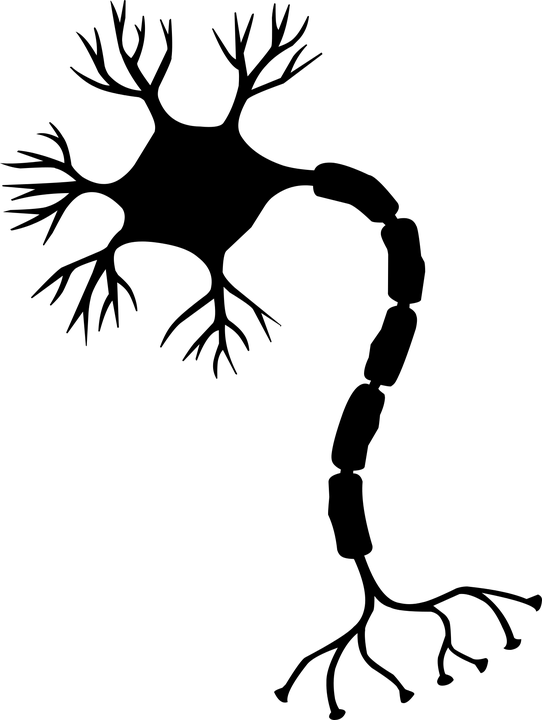
\includegraphics[width=0.5\linewidth]{neurona.png}};
		\draw[color=black] (-2.5,2.2) node {Dendritas};
		\draw[color=black] (1.2,1.6) node {Axón};
		\draw[color=white] (-0.6,1.3) node {\textbf{Soma}};
		\draw[color=black] (0,-3) node {Botones Sinápticos};
	\end{tikzpicture}
\end{center}
Actualmente se sabe que las neuronas en el cerebro humano se encargan de hacer posible el aprendizaje conectándose entre ellas para aprender de los estímulos que reciben.  Lo que básicamente ocurre es que por medio de las \textbf{dendritas}, una neurona es estimulada o excitada mediante impulsos eléctricos procesados en el cuerpo de la neurona o \textbf{soma}. Cuando en el soma se alcanza un cierto umbral, se dispara o activa, pasando la señal al \textbf{axón} que envía la información del soma para luego comunicarse con otras neuronas por medio de los \textbf{botones sinápticos}.

Se ha observado que las neuronas aprenden de la experiencia para responder a nueva información. Además, trabajan en conjunto como un sistema cuyas partes no tienen las mismas propiedades que el sistema completo.
%%%%%%%%%%%%%%%%%%%%%%%%%%%%%%%%%%%%%%%%%%%%%%%%%%%%%%%%%%%%%%%%%%%%%%%%%%%%%%%%%%%%%%%%%%%%%%%%%%%%%%%%%%%%%%%
%%%%%%%%%%%%%%%%%%%%%%%%%%%%%%%%%%%%%%%%%%%%%%%%%%%%%%%%%%%%%%%%%%%%%%%%%%%%%%%%%%%%%%%%%%%%%%%%%%%%%%%%%%%%%%%
\section{Perceptrón como Modelo Matemático}
%%%%%%%%%%%%%%%%%%%%%%%%%%%%%%%%%%%%%%%%%%%%%%%%%%%%%%%%%%%%%%%%%%%%%%%%%%%%%%%%%%%%%%%%%%%%%%%%%%%%%%%%%%%%%%%
%%%%%%%%%%%%%%%%%%%%%%%%%%%%%%%%%%%%%%%%%%%%%%%%%%%%%%%%%%%%%%%%%%%%%%%%%%%%%%%%%%%%%%%%%%%%%%%%%%%%%%%%%%%%%%%
\begin{defi}
	Un \textbf{perceptrón} o neurona $ \mathcal{N} $ es un programa que recibe una o más entradas, externas o de otras neuronas, para luego combinarlas y producir una salida.
	
	Matemáticamente, un perceptrón que consta de $ n $ entradas, recibe información de vectores $ n- $ dimensionales $ (x_1, x_2, \dots, x_p) $  a los que se les denomina \textbf{vectores de entrada} para producir vectores de salida (uno por cada vector de entrada).  En este momento se considerarán neuronas cuya salida sea un número real.
\end{defi}

Para un vector de entrada fijo $ x=(x_1, x_2, \dots, x_n)\in\mathbb{R}^n $ se produce una salida $ y\in\mathbb{R} $, como se ilustra en el siguiente diagrama.
\selectlanguage{USenglish}
\begin{center}
	\definecolor{ffqqqq}{rgb}{1,0,0}
	\definecolor{aqaqaq}{rgb}{0.6274509803921568,0.6274509803921568,0.6274509803921568}
	\definecolor{cqcqcq}{rgb}{0.7529411764705882,0.7529411764705882,0.7529411764705882}
	\begin{tikzpicture}[line cap=round,line join=round,>=triangle 45,x=1cm,y=1cm]
		\clip(-2,0) rectangle (5.7,5);
		%%%%%%%%%%%%%%%%%%%%% I N P U T S %%%%%%%%%%%%%%%%%%%%%
		\draw [line width=0.5pt] (-0.5,2.75) rectangle (0, 3.25);
		\draw [line width=0.5pt] (-0.5,0.75) rectangle (0, 1.25);
		%%%% PESOS
		\draw [->,line width=0.5pt] (0,3) -- (1,2);
		\draw [->,line width=0.5pt] (0,1) -- (1,2);
		%BIAS
		\draw [line width=0.5pt] (0.71,4.5) -- (1.8,4.5);
		\draw [->,line width=0.5pt] (1.8,4.5) -- (1.8,3);
		\draw[color=black] (0.5,4.5) node {\boxed{b}};
		
		%NEURONA
		\draw [line width=1pt] (2,2) circle (1cm);
		
		%%%% SALIDAS
		\draw [->,line width=0.5pt] (3,2) -- (4,2);
		\draw[color=black] (-0.25,3) node {$ x_1 $};
		\draw[color=black] (-0.25,2) node { \vdots };
		\draw[color=black] (-0.25,1) node {$ x_n $};
		\draw[color=black] (3.8,2.3) node {$y$};
		\draw[color=black] (2,2) node {\small{información}};
	\end{tikzpicture}
\end{center}
\begin{obs}
	Se incorpora un término $ b $ denominado \textbf{sesgo o bias} $ b\in\{0, 1\} $, que representa una carga eléctrica acumulada de un proceso realizado con anterioridad. En este sentido, $ b=0 $ representa que la neurona no se activó y $ b=1 $ diría que se activó. Más adelante se verá que este término sirve de ``soporte'' para la información que recibe el cuerpo de la neurona.
\end{obs}

En el modelo biológico, la intensidad depende del impulso eléctrico asociado a las conexiones entre neuronas. En este modelo matemático, lo anterior quiere decir que cada uno de los componentes de un vector de entrada dado, tiene  asociado un número real que pondera esta información al que sen le llamará \textbf{peso}.

\begin{defi}
	Se toma una neurona $ \mathcal{N} $ con $ n\in\mathbb{N} $ entradas. El \textbf{vector de pesos} o vector de nivel de influencia $ w\in\mathbb{R}^n $,  asociado a $ \mathcal{N} $, es el vector que pondera a cada uno de los vectores de entrada.
	
	Esto quiere decir que, para un vector de pesos $ w=(w_1, \dots, w_n) $ fijo y un vector de entrada dado $ x=(x_1, \dots, x_n) $, la información de $ x $ que llega a  $ \mathcal{N} $ está dada por
	\begin{equation*}
		x\cdot w=\sum_{i=1}^{n} w_i x_i.
	\end{equation*}
\end{defi}

\textbf{Nota}. A cada una de las entradas de un vector de pesos se le llama peso.

Al término bias también se le asocia un peso. Así que la información total que llega a una neurona $ \mathcal{N} $, de un vector de entrada $ x=(x_1, \dots, x_n) $ y un término $ b $, está dada por
\begin{equation}\label{trans}
	h=x\cdot w+w_b b=\sum_{i=1}^{n} w_i x_i+w_b b.
\end{equation}

\begin{obs}
	Por convención $ w_i $ se toma en $ [-1,1] $. Dado $ x=(x_1,\dots, x_n)\in\mathbb{R}^{n} $, tal que $ x_i\geq0 $, para todo $ 1\leq i \leq n $,
	\begin{enumerate}
		\item Si $ w_i=0 $, la entrada $ x_i $ no llega a la neurona.
		\item Si $ w_i=1 $, entrada $ x_i $ llega completa.
		\item Si $ w_i\in (0,1) $, la entrada $ x_i $ llega a la neurona pero con menor intensidad.
		\item Si $ w_i\in (-1,0) $, hay un robo de información.
	\end{enumerate}
\end{obs}

\begin{defi}
	Una \textbf{función de activación} es una función $ f $ que calcula la salida de una neurona a partir de los valores de entrada. Es decir, el argumento de $ f $ es (\ref{trans}). 
\end{defi}

\begin{obs}
	Cuando recién se inventó el modelo de perceptrón, las funciones de activación se escogían binarias. Es decir, $ f(x)\in\{0,1\} $, donde si $ f(x)=0 $, la neurona no se activa y si $ f(x)=1 $, la neurona se activa.
\end{obs}

De esta manera se obtiene la salida de la neurona $ y\in\mathbb{R} $. 

El siguiente esquema resume las etapas del transito de la información en una neurona matemática.
\begin{center}
	\definecolor{ffqqqq}{rgb}{1,0,0}
	\definecolor{aqaqaq}{rgb}{0.6274509803921568,0.6274509803921568,0.6274509803921568}
	\definecolor{cqcqcq}{rgb}{0.7529411764705882,0.7529411764705882,0.7529411764705882}
	\begin{tikzpicture}[line cap=round,line join=round,>=triangle 45,x=1cm,y=1cm]
		\clip(-2,0) rectangle (4.8,5);
		%%%%%%%%%%%%%%%%%%%%% I N P U T S %%%%%%%%%%%%%%%%%%%%%
		\draw [line width=0.5pt] (-0.5,2.75) rectangle (0, 3.25);
		\draw [line width=0.5pt] (-0.5,0.75) rectangle (0, 1.25);
		%%%% PESOS
		\draw [->,line width=0.5pt] (0,3) -- (1,2);
		\draw [->,line width=0.5pt] (0,1) -- (1,2);
		%BIAS
		\draw [line width=0.5pt] (0.71,4.5) -- (1.8,4.5);
		\draw [->,line width=0.5pt] (1.8,4.5) -- (1.8,3);
		%%%% SALIDAS
		\draw [->,line width=0.5pt] (3,2) -- (4.5,2);
		%BIAS
		\draw[color=black] (0.5,4.5) node {\boxed{b}};
		%NEURONA
		\draw [line width=1pt] (2,2) circle (1cm);
		\draw [shift={(2,2)},line width=1pt,fill=ffqqqq,fill opacity=0.35]  plot[domain=1.5707963267948965:4.71238898038469,variable=\t]({1*1*cos(\t r)+0*1*sin(\t r)},{0*1*cos(\t r)+1*1*sin(\t r)});
		\begin{scriptsize}
			\draw[color=black] (-0.25,3) node {$ x_1 $};
			\draw[color=black] (-0.25,2) node { \vdots };
			\draw[color=black] (-0.25,1) node {$ x_n $};
			\draw[color=black] (0.5,3.1) node {$w_1$};
			\draw[color=black] (0.5,0.9) node {$w_n$};
			\draw[color=black] (1.5,2) node {$h:\Sigma $};
			\draw[color=black] (2.5,2) node {$f(h)$};
			\draw[color=black] (3.6,2.2) node {$f(h)=y$};
			
		\end{scriptsize}
	\end{tikzpicture}
\end{center}
%%%%%%%%%%%%%%%%%%%%%%%%%%%%%%%%%%%%%%%%%%%%%%%%%%%%%%%%%%%%%%%%%%%%%%%%%%%%%%%%%%%%%%%%%%%%%%%%%%%%%%%%%%%%%%%
%%%%%%%%%%%%%%%%%%%%%%%%%%%%%%%%%%%%%%%%%%%%%%%%%%%%%%%%%%%%%%%%%%%%%%%%%%%%%%%%%%%%%%%%%%%%%%%%%%%%%%%%%%%%%%%
\subsection{Aprendizaje de una Neurona}
\begin{defi}
	Sea $ \mathcal{N} $ una neurona con $ n $ entradas. Dados un conjunto de vectores de entrada  $x_1, \dots , x_k\in\mathbb{R}^n $ y un conjunto de salidas $ y_1, \dots, y_k\in\mathbb{R}$, se define un \textbf{conjunto de entrenamiento} o \textbf{conjunto de patrones} como el conjunto de todos los pares  $ (x_i, y_i) $ para $ 1\leq i \leq k $. Es decir, un conjunto de aprendizaje es un conjunto de vectores de entrada de los que ya se conoce su salida. 
	\begin{eqnarray*}
		x_1=(x_{1_1},\dots, x_{n_1} ) &\to& y_1^d,\\
		x_2=(x_{1_2},\dots, x_{n_2} ) &\to& y_2^d,\\
		x_3=(x_{1_3},\dots, x_{n_3} ) &\to& y_3^d,\\
		&\vdots& \\
		x_k=(x_{1_k},\dots, x_{n_k} ) &\to& y_k^d,
	\end{eqnarray*}
	donde el superíndice $ d $ denota que tal salida es la ``deseada''.
\end{defi}
Por ejemplo, un conjunto de aprendizaje podría estar dado por vectores de entrada que representen imágenes de perros o gatos y la salida a cada uno de estos vectores de entrada será  uno  si corresponde a un perro o cero si corresponde a un gato.
%%%%%%%%%%%%%%%%%%%%%%%%%%%%%%%%%%%%%%%%%%%%%%%%%%%%%%%%%%%%%%%%%%%%%%%%%%%%%%%%%%%%%%%%%%%
\begin{center}
	\begin{tikzpicture}
		\draw  (0,0) node {\boxed{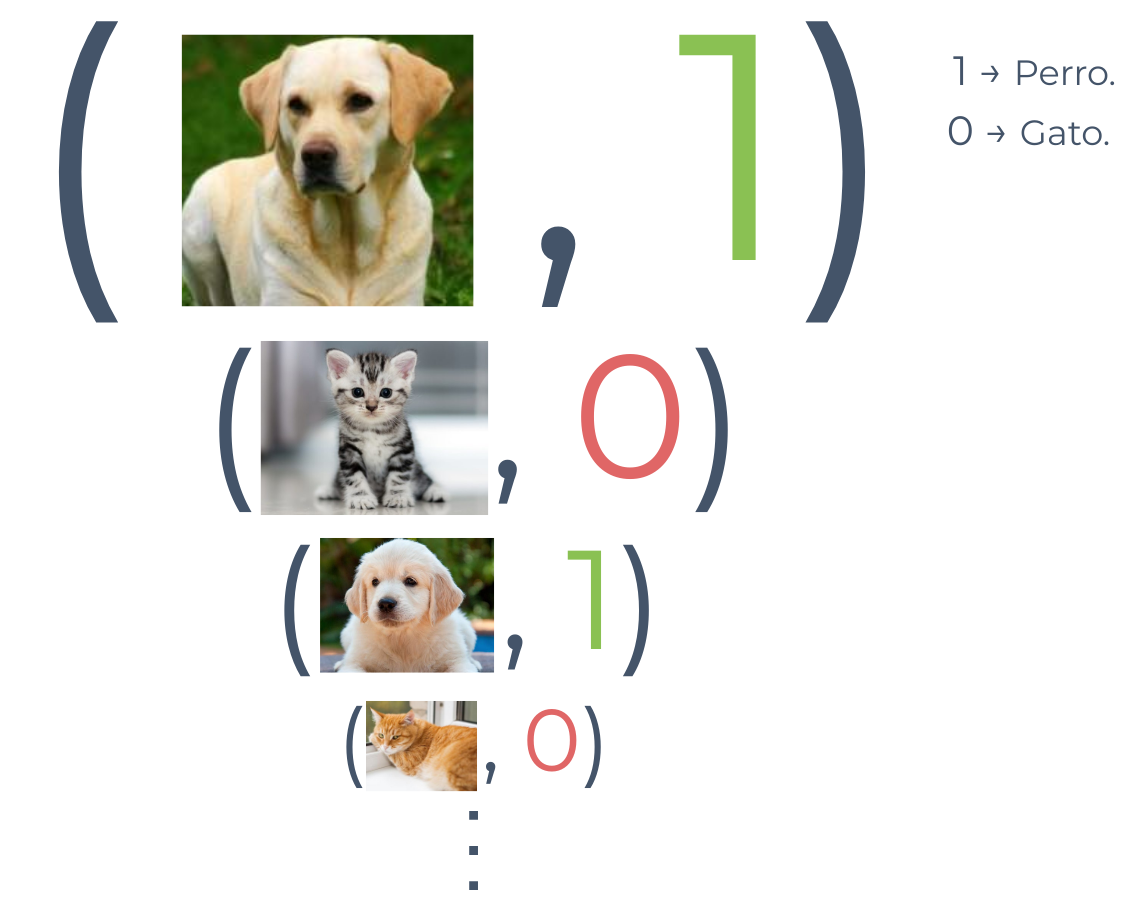
\includegraphics[width=0.6\linewidth]{pg.png}}};
	\end{tikzpicture}
\end{center}
%%%%%%%%%%%%%%%%%%%%%%%%%%%%%%%%%%%%%%%%%%%%%%%%%%%%%%%%%%%%%%%%%%%%%%%%%%%%%%%%%%%%%%%%%%%

Nótese que, en general,  dada una neurona $ \mathcal{N} $ y un conjunto de aprendizaje, se desconoce el vector de pesos tal que, al pasar la información por $ \mathcal{N} $, dé la salida $ y_i $ del conjunto de aprendizaje. Por lo tanto, la meta es encontrar el vector de pesos $ w=(w_1, \dots, w_n) $ y el peso $ w_b $ para que, dado un Conjunto de Aprendizaje, cuando cada uno de los vectores de entrada $ x_i \in\mathbb{R}^n$ entre a $ \mathcal{N} $, dé la salida deseada $ y_i $. 

Si inicialmente se da un vector de pesos aleatorios, éste se podría iterar para que aproxime mejor las salidas deseadas.

%%%%%%%%%%%%%%%%%%%%%%%%%%%%%%%%%%%%%%%%%%%%%%%%%%%%%%%%%%%%%%%%%%%%%%%%%%%%%%%%%%%%%%%%%%%%%%%%%%%%%%%%%%%%%%%%%%%%%%%%
\begin{defi}\label{defit}
	Sea $ T\in\mathbb{N} $ un número finito de iteraciones de pesos y $ t $ tal que  $ 1\leq t \leq T $. Dado un patrón $ (x_p,y_p^d) $ de un conjunto de aprendizaje y un vector de $ w_t $ en la iteración $ t $, se denotará a la \textbf{salida producida} por $ x_p $,  en la iteración $ t $, como $ y_p^t $.
\end{defi}
%%%%%%%%%%%%%%%%%%%%%%%%%%%%%%%%%%%%%%%%%%%%%%%%%%%%%%%%%%%%%%%%%%%%%%%%%%%%%%%%%%%%%%%%%%%%%%%%%%%%%%%%%%%%%%%%%%%%%%%%

\begin{defi}
	Se dirá que una neurona \textbf{está aprendiendo} si, dadas las suposiciones de la Definición \ref{defit} y una función de error $ e_t(y_p^d, y_p^t )>0 $, se cumple que 
	\[ e_{t+1}\leq e_t . \]
	
	Una neurona es capaz de modelar un conjunto de aprendizaje dado variando los pesos, como se verá a continuación. 
	
	\textbf{Nota}. Hasta ahora, no se ha dado un método que diga cómo ajustar los pesos iniciales.
\end{defi}
%%%%%%%%%%%%%%%%%%%%%%%%%%%%%%%%%%%%%%%%%%%%%%%%%%%%%%%%%%%%%%%%%%%%%%%%%%%%%%%%%%%%%%%%%%%%%%%%%%%%%%%%%%%%%%%
%%%%%%%%%%%%%%%%%%%%%%%%%%%%%%%%%%%%%%%%%%%%%%%%%%%%%%%%%%%%%%%%%%%%%%%%%%%%%%%%%%%%%%%%%%%%%%%%%%%%%%%%%%%%%%%
\subsection{Ejemplos con una neurona}
%%%%%%%%%%%%%%%%%%%%%%%%%%%%%%%%%%%%%%%%%%%%%%%%%%%%%%%%%%%%%%%%%%%%%%%%%%%%%%%%%%%%%%%%%%%%%%%%%%%%%%%%%%%%%%%
%%%%%%%%%%%%%%%%%%%%%%%%%%%%%%%%%%%%%%%%%%%%%%%%%%%%%%%%%%%%%%%%%%%%%%%%%%%%%%%%%%%%%%%%%%%%%%%%%%%%%%%%%%%%%%%
\begin{ej} PUERTA AND
	
	Se quiere que una neurona modele la tabla de verdad de la conjunción, dada por
	\begin{eqnarray*}
		x_1=(0, 0) &\to& y_1^d=0,\\
		x_2=(0, 1) &\to& y_2^d=0,\\
		x_3=(1, 0) &\to& y_3^d=0,\\
		x_4=(1, 1) &\to& y_4^d=1.
	\end{eqnarray*}
	Donde 0 representa falso y 1 verdadero. Se toma $ b=1 $ y se dan los siguientes pesos iniciales
	\begin{eqnarray*}
		w&=&(1, 1),\\
		w_b&=&1.
	\end{eqnarray*}
	
	Se procede a ajustar al tanteo. Una combinación de pesos que hacen posible este resultado es
	\begin{center}
		\definecolor{ffqqqq}{rgb}{1,0,0}
		\definecolor{aqaqaq}{rgb}{0.6274509803921568,0.6274509803921568,0.6274509803921568}
		\definecolor{cqcqcq}{rgb}{0.7529411764705882,0.7529411764705882,0.7529411764705882}
		\begin{tikzpicture}[line cap=round,line join=round,>=triangle 45,x=1cm,y=1cm]
			\clip(-2,0) rectangle (5.7,5);
			%%%% ENTRADAS
			\draw[color=black] (-1,2) node {$ \begin{matrix}
					x_1=(0, 0)\\
					x_2=(0, 1)\\
					x_3=(1, 0)\\
					x_4=(1, 1)\\
				\end{matrix} $};
			%%%% PESOS
			\draw[color=black] (1,3.2) node {$w_{1}=0.5$};
			\draw [->,line width=0.5pt] (0,3) -- (1,2);
			
			\draw[color=black] (1,0.7) node {$w_{2}=0.5$};
			\draw [->,line width=0.5pt] (0,1) -- (1,2);
			
			\draw[color=black] (3,3.75) node {$w_{b}=-0.9$};
			\draw [line width=0.5pt] (0.975,4.5) -- (2,4.5);
			\draw [->,line width=0.5pt] (2,4.5) -- (2,3);
			
			%BIAS
			\draw[color=black] (0.5,4.5) node {\boxed{$b=1$}};
			
			%NEURONA
			\draw [line width=1pt] (2,2) circle (1cm);
			\draw[color=black] (2,2) node {$w\cdot x_i-0.9$};
			
			%%%% SALIDAS
			\draw [->,line width=0.5pt] (3,2) -- (4,2);
			\draw[color=black] (4.6,2) node {$ \begin{matrix}
					y_1^d=0\\
					y_2^d=0\\
					y_3^d=0\\
					y_4^d=1\\
				\end{matrix} $};
		\end{tikzpicture}
	\end{center}
	con la función de activación
	\[ f(t)=\left\{\begin{matrix} 
		0,&\textup{ si }t<0,\\
		1,&\textup{ si }t\geq0\\
	\end{matrix}\right. \]
	
	En realidad, para este ejemplo, 
	\begin{equation}\label{recta}
		0.5 x_{i_1} +0.5 x_{i_2}-0.9=0 
	\end{equation} 
	es una recta que separa en dos clases a las salidas deseadas en el plano $ x_{i_1} x_{i_2} $, como se observa en la siguiente figura
	\begin{center}
		\begin{tikzpicture}[scale = 4]
			\draw[->, line width=0.5pt] (0,0) -- (1,0);
			\draw [->, line width=0.5pt] (0,0) -- (0,1);
			\draw [color=blue] (0.1,0.1) node {0};
			\draw [color=blue] (0.9,0.1) node {0};
			\draw [color=blue] (0.1,0.9) node {0};
			\draw [color=red] (0.9,0.9) node {1};
			\draw [color=black, domain=0.2:1, line width=0.5pt] plot(\x, {-0.25*\x+1} );
		\end{tikzpicture}
	\end{center}
	
	Así que, para una neurona con solo dos pesos y salidas binarias, el problema de encontrar una combinación de pesos se convierte en encontrar un separador lineal del conjunto de puntos en el espacio de patrones en dos clases.
	\begin{obs}
		La combinación de pesos que hace posible la separabilidad lineal, no es única. Además, $ w_b $ funciona como el término independiente en (\ref{recta}), el cual permite desplazar la recta de manera vertical.
	\end{obs}
\end{ej}
%%%%%%%%%%%%%%%%%%%%%%%%%%%%%%%%%%%%%%%%%%%%%%%%%%%%%%%%%%%%%%%%%%%%%%%%%%%%%%%%%%%%%%%%%%%%%%%%%%%%%%%%%%%%%%%%%%%%%%%%%%%%%%%%%%%%%%%%%%%
\begin{ej}PUERTA XOR.
	El siguiente conjunto de aprendizaje representa la tabla de verdad de la disyunción exclusiva. Nuevamente, 0 representa falso y 1 verdadero.
	\begin{eqnarray*}
		x_1=(0, 0) &\to& y_1^d=0\\
		x_2=(0, 1) &\to& y_2^d=1\\
		x_3=(1, 0) &\to& y_3^d=1\\
		x_4=(1, 1) &\to& y_4^d=0.
	\end{eqnarray*}
	Así que se quiere encontrar una recta que separe en dos clases al diagrama
	\begin{center}
		\begin{tikzpicture}[scale = 4]
			\draw[->, line width=0.5pt] (0,0) -- (1,0);
			\draw [->, line width=0.5pt] (0,0) -- (0,1);
			\draw [color=blue] (0.1,0.1) node {0};
			\draw [color=red] (0.9,0.1) node {1};
			\draw [color=red] (0.1,0.9) node {1};
			\draw [color=blue] (0.9,0.9) node {0};
		\end{tikzpicture}
	\end{center}
	
	Lo cual no es posible con una sola recta pero sí con dos. De manera intuitiva, esto dice que si se agrega otra neurona al programa, se podría separar linealmente a este conjunto de patrones. Marvin Minksy en su libro Perceptrons \cite{4} en 1969 escribió sobre las limitaciones de una neurona, pues es incapaz de trascender a la separalibilidad lineal. Aunque Minsky habló sobre la posibilidad de agregar más neuronas para resolver el problema de la separabilidad lineal, descalificó este método, argumentando que no se encontraría un algoritmo para encontrar un vector de pesos adecuado que hiciera que las neuronas aprendieran. Como Minsky tenía un gran prestigio en la política científica, todas las investigaciones en cómputo neuronal se detuvieron alrededor de 1970. 
	
	Sin embargo, en 1987, David Rumelhart y Francis Crick, en su libro Procesos Paralelos Distribuídos \cite{5} escribieron sobre redes de neuronas cuya capacidad colectiva no es igual a la suma de las capacidades individuales. Además, mostraron un algoritmo para entrenar una red neuronal a partir de un conjunto de aprendizaje, que ajustó los pesos de manera adecuada.
	
	
	Dicho algoritmo se llama Retropropagación, del cual se hablará en la Sección \ref{bp}.
\end{ej}
%%%%%%%%%%%%%%%%%%%%%%%%%%%%%%%%%%%%%%%%%%%%%%%%%%%%%%%%%%%%%%%%%%
\section{Redes Neuronales Artificiales}
\begin{defi}\label{d1}
	Una \textbf{Red Neuronal Prealimentada} consiste de una capa de entrada ($ X $ con $ N_0 \in\mathbb{N}$ entradas ordenadas) y dos capas de neuronas ordenadas ($ V $ con $ N_1 \in\mathbb{N}$ neuronas, $ Y $ con $ N_2 \in\mathbb{N}$ neuronas) llamadas capa oculta y capa de salida, respectivamente, tales que sólo existen conexiones hacia adelante entre neuronas de capas adyacentes.
	
	\textbf{Nota}. La definición anterior indica que, en una red neuronal artificial de este tipo, no se permiten ciclos ni conexiones entre neuronas de la misma capa.
\end{defi}
\vspace{-.5em}
La siguiente figura representa una red neuronal como en la Definición \ref{d1}.
%%%%%%%%%%%%%%%%%%%%%%%%%%%%%%%%%%%%%%%%%%%%%%%%%%%%%%%%%%%%%%%%%%%%%%%%%%%%%%%%%%%%%%%%%%%%%%%%%%%%%%%%%%%%%%%
\begin{center}
	\definecolor{aqaqaq}{rgb}{0.6274509803921568,0.6274509803921568,0.6274509803921568}
	\begin{tikzpicture}[line cap=round,line join=round,>=triangle 45,x=0.55cm,y=0.55cm]
		\clip(-2.45,-4) rectangle (10.55,8);
		%%%%%%%%%%%%%%% N E U R O N S %%%%%%%%%%%%%%%%
		%layer 0
		\draw [line width=1pt] (-1.8,5.2) rectangle (-0.2,6.8);
		\draw [line width=1pt] (-1.8,1.2) rectangle (-0.2,2.8);
		\draw [line width=1pt] (-1.8,-2.8) rectangle (-0.2,-1.2);
		%layer 1
		\draw [line width=1pt] (4,6) circle (0.55cm);
		\draw [line width=1pt] (4,2) circle (0.55cm);
		\draw [line width=1pt] (4,-2) circle (0.55cm);
		%layer 2
		\draw [line width=1pt] (9,6) circle (0.55cm);
		\draw [line width=1pt] (9,2) circle (0.55cm);
		\draw [line width=1pt] (9,-2) circle (0.55cm);
		%%%%%%%%%%%%%%%%%%%%%%%%%%%%%%%%%%%%%%%%%%%%%%%%%%%%%%%%%%% W E I G H T S %%%%%%%%%%%%%%%%%%%%%%%%%%%%%%%%%%%%%%%%%%%%%%%%%%%%%%%%%%%
		%weights 01
		%w00
		\draw [->,line width=0.5pt] (-0.2,6) -- (3,6);
		%w01
		\draw [->,line width=0.5pt] (-0.2,5.2) -- (3.4,2.8);
		%w02
		\draw [->,line width=0.5pt] (-1,5.2) -- (4,-1);
		%%%%%%%%%%%%%%%%%%%%%%%%%%%%%%%%%%%%%%%%%%%%%%%%%%%%%%%%%%%%%%%%%%%%%%%%%%%%%%%%%%%%%%%%%%%%%%%%%%%%%%%%%%%%%%%%%%%%%%%%%%%%%%%%%%%%%
		%w10
		\draw [->,line width=0.5pt] (-0.2,2.8) -- (3.292893218813452,5.292893218813452);
		%w11
		\draw [->,line width=0.5pt] (-0.2,1.2) -- (3.4,-1.2);
		%w12
		\draw [->,line width=0.5pt] (-0.2,2) -- (3,2);
		%%%%%%%%%%%%%%%%%%%%%%%%%%%%%%%%%%%%%%%%%%%%%%%%%%%%%%%%%%%%%%%%%%%%%%%%%%%%%%%%%%%%%%%%%%%%%%%%%%%%%%%%%%%%%%%%%%%%%%%%%%%%%%%%%%%%%
		%w20
		\draw [->,line width=0.5pt] (-1,-1.2) -- (4,5);	
		%w21
		\draw [->,line width=0.5pt] (-0.2,-1.2) -- (3.292893218813452,1.3);
		%w22
		\draw [->,line width=0.5pt] (-0.2,-2) -- (3,-2);
		%%%%%%%%%%%%%%%%%%%%%%%%%%%%%%%%%%%%%%%%%%%%%%%%%%%%%%%%%%%%%%%%%%%%%%%%%%%%%%%%%%%%%%%%%%%%%%%%%%%%%%%%%%%%%%%%%%%%%%%%%%%%%%%%%%%%%
		%weights 12
		\draw [->,line width=0.5pt] (5,6) -- (8,6);
		\draw [->,line width=0.5pt] (4.707106781186548,5.292893218813452) -- (8.3,2.707106781186548);
		\draw [->,line width=0.5pt] (4,5) -- (9,-1);
		\draw [->,line width=0.5pt] (4.707106781186548,2.707106781186548) -- (8.3,5.3);
		\draw [->,line width=0.5pt] (5,2) -- (8,2);
		\draw [->,line width=0.5pt] (4.7,1.3) -- (8.3,-1.3);
		\draw [->,line width=0.5pt] (5,-2) -- (8,-2);
		\draw [->,line width=0.5pt] (4.707106781186548,-1.3) -- (8.3,1.3);
		\draw [->,line width=0.5pt] (4,-1) -- (9,5);
		%%%%%%%%%%%%%%%%%%%%%%%%%%%%%%%%%%%%%%%%%%%%%%%%%%%%%%%%%%%%%%%%%%%%%%%%%%%%%%%%%%%%%%%%%%%%%%%%%%%%%%%%%%%%%%%%%%%%%%%%%%%%%%%%%%%%%
		%%%%%%%%%%%%%%%%%%%%%%%%%%%%%%%%%%%%%%%%%%%%%%%%%%%%%%% R E C T A N G L E S %%%%%%%%%%%%%%%%%%%%%%%%%%%%%%%%%%%%%%%%%%%%%%%%%%%%%%%%%
		%lL A Y E R 0
		\draw [line width=0.5pt] (-2.4,7.4) -- (0.6,7.4);
		\draw [line width=0.5pt] (-2.4,7.4) -- (-2.4,-3.5);
		\draw [line width=0.5pt] (0.6,7.4) -- (0.6,-3.5);
		\draw [line width=0.5pt] (-2.4,-3.5) -- (0.6,-3.5);
		%L A Y E R 1
		\draw [line width=0.5pt] (2.6,7.4) -- (5.5,7.4);
		\draw [line width=0.5pt] (2.6,7.4) -- (2.6,-3.5);
		\draw [line width=0.5pt] (5.5,7.4) -- (5.5,-3.5);
		\draw [line width=0.5pt] (2.6,-3.5) -- (5.5,-3.5);
		%L A Y E R 2
		\draw [line width=0.5pt] (7.6,7.4) -- (10.5,7.4);
		\draw [line width=0.5pt] (7.6,7.4) -- (7.6,-3.5);
		\draw [line width=0.5pt] (10.5,7.4) -- (10.5,-3.5);
		\draw [line width=0.5pt] (7.6,-3.5) -- (10.5,-3.5);
		%T A G S
		\begin{scriptsize}
			\draw[color=black] (0.0731375855871272,7) node {$x_{i_0}$};
			\draw[color=black] (-1,0) node {\Huge\vdots};
			\draw[color=black] (5,7) node {$v_{i_1}$};
			\draw[color=black] (4,0) node {\Huge\vdots};
			\draw[color=black] (10, 7) node {$y_{i_2}$};
			\draw[color=black] (9,0) node {\Huge\vdots};
			\draw[color=black] (1.6,6.439428935813765) node {$w_{i_0 i_1}$};
			\draw[color=black] (6.48,6.453980953984906) node {$w_{i_1 i_2}$};
			\draw[color=black] (-1,7.7) node {\textbf{$X$}};
			\draw[color=black] (4,7.7) node {\textbf{$V$}};
			\draw[color=black] (9,7.7) node {\textbf{$Y$}};
		\end{scriptsize}
	\end{tikzpicture}
\end{center}
%%%%%%%%%%%%%%%%%%%%%%%%%%%%%%%%%%%%%%%%%%%%%%%%%%%%%%%%%%%%%%%%%%%%%%%%%%%%%%%%%%%%%%%%%%%%%%%%%%%%%%%%%%%%%%%%%%%%%%%%%%%%%%%%%%%%%%%%%%%%%
Nótese que el segundo subíndice indica la capa a la que pertenece la neurona en cuestión.
%%%%%%%%%%%%%%%%%%%%%%%%%%%%%%%%%%%%%%%%%%%%%%%%%%%%%%%%%%%%%%%%%%%%%%%%%%%%%%%%%%%%%%%%%%%%%%%%%%%%%%%%%%%%%%%
%%%%%%%%%%%%%%%%%%%%%%%%%%%%%%%%%%%%%%%%%%%%%%%%%%%%%%%%%%%%%%%%%%%%%%%%%%%%%%%%%%%%%%%%%%%%%%%%%%%%%%%%%%%%%%%
\textbf{Funciones de Activación}

\noindent
%%%%%%%%%%%%%%%%%%%%%%%%%%%%%%%%%%%%%%%%%%%%%%%%%%%%%%%%%%%%%%%%%%%%%%%%%%%%%%%%%%%%%%%%%%%%%%%%%%%%%%%%%%%%%%%
%%%%%%%%%%%%%%%%%%%%%%%%%%%%%%%%%%%%%%%%%%%%%%%%%%%%%%%%%%%%%%%%%%%%%%%%%%%%%%%%%%%%%%%%%%%%%%%%%%%%%%%%%%%%%%%
La intensidad de la información que pasa de la capa de entrada a la neurona $ i_1 $ de la capa oculta está dada por
\begin{equation}\label{1}
	h_{i_1}=\displaystyle\sum_{i_0} x_{i_0} w_{i_1}+\theta_{i_1}.
\end{equation}
Donde $\theta_{i_1}$ es el bias correspondiente a la neurona con la etiqueta $ i_1 $. En términos geométricos, este término permite desplazar verticalmente al hiper-plano definido por los pesos.
%%%%%%%%%%%%%%%%%%%%%%%%%%%%%%%%%%%%%%%%%%%%%%%%%%%%%%%%%%%%%%%%%%%%%%%%%%%%%%%%%%%%%%%%%%%%%%%%%%%%%%%%%%%%%%%%%%%%%%%%%%%%%%%%%%%%%
\begin{center}
	\boxed{\begin{tikzpicture}[scale = 0.4]
			\draw[->, line width=0.5pt] (-5,0) -- (5,0);
			\draw [->, line width=0.5pt] (0,-3) -- (0,6);
			\draw [color=black, domain=-4:5, line width=0.5pt] plot(\x, {\x+1} );
			\draw [color=red, domain=-5:5, line width=0.5pt] plot(\x, {\x+2} );
			\draw [color=blue, domain=-5:4, line width=0.5pt] plot(\x, { \x+3} );
	\end{tikzpicture}}
\end{center}
%%%%%%%%%%%%%%%%%%%%%%%%%%%%%%%%%%%%%%%%%%%%%%%%%%%%%%%%%%%%%%%%%%%%%%%%%%%%%%%%%%%%%%%%%%%%%%%%%%%%%%%%%%%%%%%%%%%%%%%%%%%%%%%%%%%%%

Intuitivamente (\ref{1}) dice que la información recibida en una neurona de la capa oculta es la suma de la información de cada neurona de la capa anterior con la intensidad que está dada por el respectivo peso. Una vez que se tiene (\ref{1}), este término pasa a través de una función de activación, análogo al modelo de una sola neurona.
\[f \left(\displaystyle\sum_{i_0} x_{i_0} w_{i_1}+\theta_{i_1}\right)=f(h_{i_1}).\]

Para la función de activación, el término $ \theta_{j_1} $ permite trasladar la función de activación horizontalmente.
%%%%%%%%%%%%%%%%%%%%%%%%%%%%%%%%%%%%%%%%%%%%%%%%%%%%%%%%%%%%%%%%%%%%%%%%%%%%%%%%%%%%%%%%%%%%%%%%%%%%%%%%%%%%%%%%%%%%%%%%%%%%%%%%%%%%%
\begin{center}
	\boxed{\begin{tikzpicture}[scale = 0.4]
			\draw[->, line width=0.5pt] (-7,0) -- (7,0);
			\draw [->, line width=0.5pt] (0,-3) -- (0,6);
			\draw [color=black, domain=-7:7, line width=0.5pt] plot(\x, {4/(1+exp(-\x))} );
			\draw [color=red, domain=-7:7, line width=0.5pt] plot(\x, {4/(1+exp(-\x-2))} );
			\draw [color=blue, domain=-7:7, line width=0.5pt] plot(\x, {4/(1+exp(-\x++2))} );
	\end{tikzpicture}}
\end{center}
En resumen,
\begin{eqnarray*}\label{rn}
	h_{i_1}=\displaystyle\sum_{i_0}w_{i_0i_1}x_{i_0}, & f(h_{i_1})=v_{i_1},\\
	h_{i_2}=\displaystyle\sum_{i_1}w_{i_1i_2}v_{i_1}, & f(h_{i_2})=y_{i_2}.
\end{eqnarray*}
%%%%%%%%%%%%%%%%%%%%%%%%%%%%%%%%%%%%%%%%%%%%%%%%%%%%%%%%%%%%%%%%%%%%%%%%%%%%%%%%%%%%%%%%%%%%%%%%%%%%%%%%%%%%%%%%%%%%%%%%%%%%%%%%%%%%%
%%%%%%%%%%%%%%%%%%%%%%%%%%%%%%%%%%%%%%%%%%%%%%%%%%%%%%%%%%%%%%%%%%%%%%%%%%%%%%%%%%%%%%%%%%%%%%%%%%%%%%%%%%%%%%%%%%%%%%%%%%%%%%%%%%%%%
%%%%%%%%%%%%%%%%%%%%%%%%%%%%%%%%%%%%%%%%%%%%%%%%%%%%%%%%%%%%%%%%%%%%%%%%%%%%%%%%%%%%%%%%%%%%%%%%%%%%%%%%%%%%%%%%%%%%%%%%%%%%%%%%%%%%%
Algunos ejemplos clásicos de funciones de activación son
\begin{center}
	\begin{tabular}{lc}
		\hline 
							Función					&					Gráfica								   \\ 
		\hline  
		\hline 
		%%%%%%%%%%%%%%%%%%%%%%%%%%%%%%%%%%%%%%%%%%%%%%%%%%%%%%%%%%%%%%%%%%%%%%%%%%%%%%%%%%%%%%%%%%%%%%%%%%%%%%%%%%%%%%%%%%%%%%%%%%%%%%%%%%%%%%%%%%%%%%
		$ \begin{matrix}
			Lineal \\
			f(x)=x
		\end{matrix} $              & 
		\begin{tikzpicture}[scale = 0.7]
			\draw[->, line width=0.5pt] (-1,0) -- (1,0);
			\draw[->, line width=0.5pt] (0,-1) -- (0,1);
			\draw[domain=-1:1, line width=1.5pt] plot(\x, { \x} );
		\end{tikzpicture} 									   \\
		%%%%%%%%%%%%%%%%%%%%%%%%%%%%%%%%%%%%%%%%%%%%%%%%%%%%%%%%%%%%%%%%%%%%%%%%%%%%%%%%%%%%%%%%%%%%%%%%%%%%%%%%%%%%%%%%%%%%%%%%%%%%%%%%%%%%%%%%%%%%%% 
		$ \begin{matrix}
			\textup{Límite Duro \textcolor{white}{texdsfdsgd}} \\
			f(x)=\left\{\begin{matrix}
				0, &si& x<0\\
				1, &si& x\geq 0 \\
			\end{matrix} \right.
		\end{matrix} $ &	\begin{tikzpicture}[scale = 0.7]
			\draw[->, line width=0.5pt] (-1,0) -- (1,0);
			\draw [->, line width=0.5pt] (0,-0.5) -- (0,1.5);
			\draw [domain=-1:0, line width=1.5pt] plot(\x, { 0} );
			\draw [domain=0:1, line width=1.5pt] plot(\x, { 1} );
		\end{tikzpicture} 									   \\
		%%%%%%%%%%%%%%%%%%%%%%%%%%%%%%%%%%%%%%%%%%%%%%%%%%%%%%%%%%%%%%%%%%%%%%%%%%%%%%%%%%%%%%%%%%%%%%%%%%%%%%%%%%%%%%%%%%%%%%%%%%%%%%%%%%%%%%%%%%%%%%      
		$ \begin{matrix}
			\textup{Sigmoide \textcolor{white}{texdsf}} \\
			f(x)=\dfrac{1}{1+e^{-x}}
		\end{matrix}  $
		&   \begin{tikzpicture}[scale = 0.15]
			\draw[->, line width=0.5pt] (-7,0) -- (7,0);
			\draw [->, line width=0.5pt] (0,-4) -- (0,7);
			\draw [domain=-7:7, line width=1.5pt] plot(\x, { 6/(1+exp(-\x))} );
		\end{tikzpicture} \\ 
	$ \begin{matrix}
		\textup{Tangente Hiperbólica}\\
		f(x)= \dfrac{e^x -e^{-x}}{e^x+e^{-x}}
	\end{matrix} $
	&	\begin{tikzpicture}[scale = 0.1]
			\draw[->, line width=0.5pt] (-7,0) -- (7,0);
			\draw [->, line width=0.5pt] (0,-4) -- (0,6);
			\draw [domain=-7:7, line width=1.5pt] plot(\x, { 4*(exp (\x)-exp(-\x))/(exp (\x)+exp(-\x))} );
		\end{tikzpicture}									  \\
	$ \begin{matrix}
		\textup{Lineal Positiva \textcolor{white}{texdsfst}}  \\
		f(x)=\left\{\begin{matrix}
			0, &si& x<0\\
			x, &si& x \geq 0 \\
		\end{matrix} \right.
	\end{matrix}  $ 
		& 	\begin{tikzpicture}[scale = 0.8]
			\draw[->, line width=0.5pt] (-1,0) -- (1,0);
			\draw [->, line width=0.5pt] (0,-1) -- (0,1);
			\draw [domain=-1:0, line width=1.5pt] plot(\x, { 0 } );
			\draw [domain=0:1, line width=1.5pt] plot(\x, { \x } );
		\end{tikzpicture} \\
		\hline
	\end{tabular} 
	\\
\end{center}

Además, se pueden introducir constantes $ \alpha $, $ \beta $ a una función de activación tales que 
\[ \alpha+\beta f \left(\displaystyle\sum_{i_0} x_{i_0} w_{i_1}+\theta_{i_1}\right), \]
donde  $ \alpha $ traslada a la función de activación y $ \beta $ la dilata verticalmente.
%%%%%%%%%%%%%%%%%%%%%%%%%%%%%%%%%%%%%%%%%%%%%%%%%%%%%%%%%%%%%%%%%%%%%%%%%%%%%%%%%%%%%%%%%%%%%%%%%%%%%%%%%%%%%%%%%%%%%%%%%%%%%%%%%%%%%%%%%%%%%%
\begin{obs}
	Como se vió en la primera sección, los pesos iniciales se dan de manera aleatoria y se requieren ajustarlos para que converjan a los valores esperados del conjunto de entrenamiento. Uno de los primeros métodos para hacer que una red neuronal converja es el de Backpropagation, que usa el descenso gradiente para aproximarse a un mínimo local de una función de error dada.
\end{obs}
%%%%%%%%%%%%%%%%%%%%%%%%%%%%%%%%%%%%%%%%%%%%%%%%%%%%%%%%%%%%%%%%%%%%%%%%%%%%%%%%%%%%%%%%%%%%%%%%%%%%%%%%%%%%%%%
%%%%%%%%%%%%%%%%%%%%%%%%%%%%%%%%%%%%%%%%%%%%%%%%%%%%%%%%%%%%%%%%%%%%%%%%%%%%%%%%%%%%%%%%%%%%%%%%%%%%%%%%%%%%%%%%%%%%%%%%%%%%%%%%%%%%%%%%%%%%%%%%%%%%%%%%%%%%%%%%%%%%%%%%%%%%%%%%%%%%%%%%%%%%%%%%%%%%%%%%%%%%%%%%%%%%%%%%%%%%%%
%%%%%%%%%%%%%%%%%%%%%%%%%%%%%%%%%%%%%%%%%%%%%%%%%%%%%%%%%%%%%%%%%%%%%%%%%%%%%%%%%%%%%%%%%%%%%%%%%%%%%%%%%%%%%%%
\section{Backpropagation}\label{bp}
%%%%%%%%%%%%%%%%%%%%%%%%%%%%%%%%%%%%%%%%%%%%%%%%%%%%%%%%%%%%%%%%%%%%%%%%%%%%%%%%%%%%%%%%%%%%%%%%%%%%%%%%%%%%%%%
%%%%%%%%%%%%%%%%%%%%%%%%%%%%%%%%%%%%%%%%%%%%%%%%%%%%%%%%%%%%%%%%%%%%%%%%%%%%%%%%%%%%%%%%%%%%%%%%%%%%%%%%%%%%%%%%%%%%%%%%%%%%%%%%%%%%%%%%%%%%%%%%%%%%%%%%%%%%%%%%%%%%%%%%%%%%%%%%%%%%%%%%%%%%%%%%%%%%%%%%%%%%%%%%%%%%%%%%%%%%%%
%%%%%%%%%%%%%%%%%%%%%%%%%%%%%%%%%%%%%%%%%%%%%%%%%%%%%%%%%%%%%%%%%%%%%%%%%%%%%%%%%%%%%%%%%%%%%%%%%%%%%%%%%%%%%%%
\subsection{Descenso Gradiente}
%%%%%%%%%%%%%%%%%%%%%%%%%%%%%%%%%%%%%%%%%%%%%%%%%%%%%%%%%%%%%%%%%%%%%%%%%%%%%%%%%%%%%%%%%%%%%%%%%%%%%%%%%%%%%%%
%%%%%%%%%%%%%%%%%%%%%%%%%%%%%%%%%%%%%%%%%%%%%%%%%%%%%%%%%%%%%%%%%%%%%%%%%%%%%%%%%%%%%%%%%%%%%%%%%%%%%%%%%%%%%%%
\begin{defi}
	Sea $ f: \mathbb{R}^n \to \mathbb{R} $ una función derivable. El \textbf{gradiente} de $ f $  en $ p $ es
	\[ \nabla f (p) =\left(\dfrac{\partial f(p)}{\partial x_1}, \dfrac{\partial f(p)}{\partial x_2}, \dots, \dfrac{\partial f(p)}{\partial x_n}\right)\hspace{-.3em}. \]
\end{defi}
Para una función de $ n $ variables, el gradiente es el vector normal a la curva de nivel en un punto dado.
%%%%%%%%%%%%%%%%%%%%%%%%%%%%%%%%%%%%%%%%%%%%%%%%%%%%%%%%%%%%%%%%%%%%%%%%%%%%%%%%%%%%%%%%%%%%%%%%%%%%%%%%%%%%%%%%%%%%%%%%%%%%%%%%%%%%%%%%%%%%%%
\begin{teo}
	Sea $ f: \mathbb{R}^n\to \mathbb{R} $ una funci\'on derivable. La direcci\'on donde $ f $ crece m\'as r\'apido es la direcci\'on de $ \nabla f $ (el gradiente de $ f $).
\end{teo}

\begin{cor}\label{col2}
	Bajo las condiciones del teorema anterior, $ f $ decrece más rápido en la dirección de $ -\nabla f $.
\end{cor}
%%%%%%%%%%%%%%%%%%%%%%%%%%%%%%%%%%%%%%%%%%%%%%%%%%%%%%%%%%%%%%%%%%%%%%%%%%%%%%%%%%%%%%%%%%%%%%%%%%%%%%%%%%%%%%%%%%%%%%%%%%%%%%%%%%%%%%%%%%%%%%
\begin{obs}
	Para el esquema de aprendizaje de Backpropagation se considerará la funci\'on de error (Error Cuadrático) dada por 
	\begin{equation*}
		E=\dfrac{1}{2}\sum_{i_2} (y_{i_2}-y_{i_2}^d)^2,
	\end{equation*}
	donde $ y_{i_2} $ es la salida producida por la red neuronal en la neurona con etiqueta $ i_2 $ en un momento dado y $ y_{i_2}^d $  es la salida deseada. La suma en esta función de error está multiplicada por un medio, ya que más adelante se requerirá derivar esta función con respecto a los pesos.
\end{obs}
%%%%%%%%%%%%%%%%%%%%%%%%%%%%%%%%%%%%%%%%%%%%%%%%%%%%%%%%%%%%%%%%%%%%%%%%%%%%%%%%%%%%%%%%%%%%%%%%%%%%%%%%%%%%%%%%%%%%%%%%%%%%%%%%%%%%%%%%%%%%%%
\begin{ej}
	Para la función $ f(x,y)=x^2+y^2  $ cuyo gradiente es $ \nabla f(x,y)=(2x,2y) $ se tiene el siguiente campo gradiente
	\begin{center}
		\begin{tikzpicture}
			\node[inner sep=0pt] (graph) at (0,0) {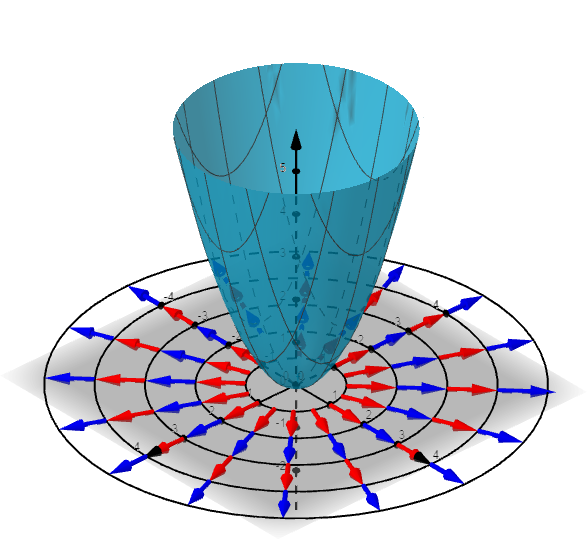
\includegraphics[width=0.8\linewidth]{gradiente.png}};
		\end{tikzpicture}
		
	\end{center}
		\begin{center}
			\definecolor{qqqqff}{rgb}{0,0,1}
			\definecolor{ffqqqq}{rgb}{1,0,0}
			\definecolor{qqwuqq}{rgb}{0,0.39215686274509803,0}
			\begin{tikzpicture}[line cap=round,line join=round,>=triangle 45,x=0.5cm,y=0.5cm]
				\begin{axis}[
					x=0.5cm,y=0.5cm,
					axis lines=middle,
					xmin=-5.5,
					xmax=5.5,
					ymin=-5.5,
					ymax=5.5,
					xtick={-4,-2,...,4},
					ytick={-4,-2,...,4},]
					\clip(-5.5,-5.5) rectangle (5.5,5.5);
					\draw [line width=1pt] (0,0) circle (0.5cm);
					\draw [line width=1pt] (0,0) circle (1.0cm);
					\draw [line width=1pt] (0,0) circle (1.5cm);
					\draw [line width=1pt] (0,0) circle (2.0cm);
					\draw [line width=1pt] (0,0) circle (2.5cm);
					\draw [->, line width=1pt,color=ffqqqq, -stealth] (-1,0) -- (-2,0);
					\draw [->,line width=1pt,color=qqqqff,-stealth] (-2,0) -- (-3,0);
					\draw [->,line width=1pt,color=ffqqqq,-stealth] (-3,0) -- (-4,0);
					\draw [->,line width=1pt,color=qqqqff,-stealth] (-4,0) -- (-5,0);
					\draw [->,line width=1pt,color=ffqqqq,-stealth] (0,1) -- (0,2);
					\draw [->,line width=1pt,color=qqqqff,-stealth] (0,2) -- (0,3);
					\draw [->,line width=1pt,color=ffqqqq,-stealth] (0,3) -- (0,4);
					\draw [->,line width=1pt,color=qqqqff,-stealth] (0,4) -- (0,5);
					\draw [->,line width=1pt,color=ffqqqq,-stealth] (1,0) -- (2,0);
					\draw [->,line width=1pt,color=qqqqff,-stealth] (2,0) -- (3,0);
					\draw [->,line width=1pt,color=ffqqqq,-stealth] (3,0) -- (4,0);
					\draw [->,line width=1pt,color=qqqqff,-stealth] (4,0) -- (5,0);
					\draw [->,line width=1pt,color=ffqqqq,-stealth] (0,-1) -- (0,-2);
					\draw [->,line width=1pt,color=qqqqff,-stealth] (0,-2) -- (0,-3);
					\draw [->,line width=1pt,color=ffqqqq,-stealth] (0,-3) -- (0,-4);
					\draw [->,line width=1pt,color=qqqqff,-stealth] (0,-4) -- (0,-5);
					%%%%%%%%%%%%%%%%%%%%%%%%%%%%%%%%%%%%%%%%%%%
					\draw [->,line width=1pt,color=ffqqqq,-stealth] (-0.7071067811865477,-0.7071067811865475) -- (-1.4142135623730954,-1.414213562373095);
					\draw [->,line width=1pt,color=qqqqff,-stealth] (-1.4142135623730954,-1.414213562373095) -- (-2.121320343559643,-2.1213203435596424);
					\draw [->,line width=1pt,color=ffqqqq,-stealth] (-2.121320343559643,-2.1213203435596424) -- (-2.8284271247461907,-2.82842712474619);
					\draw [->,line width=1pt,color=qqqqff, ,-stealth] (-2.8284271247461907,-2.82842712474619) -- (-3.5355339059327386,-3.5355339059327373);
					\draw [->,line width=1pt,color=ffqqqq, ,-stealth] (0.7071067811865475,-0.7071067811865477) -- (1.414213562373095,-1.4142135623730954);
					\draw [->,line width=1pt,color=qqqqff,-stealth] (1.414213562373095,-1.4142135623730954) -- (2.1213203435596424,-2.121320343559643);
					\draw [->,line width=1pt,color=ffqqqq,-stealth] (2.1213203435596424,-2.121320343559643) -- (2.82842712474619,-2.8284271247461907);
					\draw [->,line width=1pt,color=qqqqff,-stealth] (2.82842712474619,-2.8284271247461907) -- (3.5355339059327373,-3.5355339059327386);
					\draw [->,line width=1pt,color=ffqqqq,-stealth] (0.7071067811865477,0.7071067811865475) -- (1.4142135623730954,1.414213562373095);
					\draw [->,line width=1pt,color=qqqqff,-stealth] (1.4142135623730954,1.414213562373095) -- (2.121320343559643,2.1213203435596424);
					\draw [->,line width=1pt,color=ffqqqq,-stealth] (2.121320343559643,2.1213203435596424) -- (2.8284271247461907,2.82842712474619);
					\draw [->,line width=1pt,color=qqqqff,-stealth] (2.8284271247461907,2.82842712474619) -- (3.5355339059327386,3.5355339059327373);
					\draw [->,line width=1pt,color=ffqqqq,-stealth] (-0.7071067811865475,0.7071067811865477) -- (-1.414213562373095,1.4142135623730954);
					\draw [->,line width=1pt,color=qqqqff,-stealth] (-1.414213562373095,1.4142135623730954) -- (-2.1213203435596424,2.121320343559643);
					\draw [->,line width=1pt,color=ffqqqq,-stealth] (-2.1213203435596424,2.121320343559643) -- (-2.82842712474619,2.8284271247461907);
					\draw [->,line width=1pt,color=qqqqff,-stealth] (-2.82842712474619,2.8284271247461907) -- (-3.6530983159391743,3.6530983159391743);
					\draw [->,line width=1pt,color=ffqqqq,-stealth] (-0.3826834323650898,0.923879532511287) -- (-0.7653668647301796,1.847759065022574);
					\draw [->,line width=1pt,color=qqqqff,-stealth] (-0.7653668647301796,1.847759065022574) -- (-1.1480502970952693,2.7716385975338604);
					\draw [->,line width=1pt,color=ffqqqq,-stealth] (-1.1480502970952693,2.7716385975338604) -- (-1.5307337294603591,3.695518130045148);
					\draw [->,line width=1pt,color=qqqqff,-stealth] (-1.5307337294603591,3.695518130045148) -- (-1.9134171618254483,4.619397662556434);
					\draw [->,line width=1pt,color=ffqqqq,-stealth] (0.3826834323650898,0.9238795325112867) -- (0.7653668647301796,1.8477590650225735);
					\draw [->,line width=1pt,color=qqqqff, ,-stealth] (0.7653668647301796,1.8477590650225735) -- (1.1480502970952693,2.77163859753386);
					\draw [->,line width=1pt,color=ffqqqq,-stealth] (1.1480502970952693,2.77163859753386) -- (1.5307337294603591,3.695518130045147);
					\draw [->,line width=1pt,color=qqqqff,-stealth] (1.5307337294603591,3.695518130045147) -- (1.913417161825449,4.619397662556434);
					\draw [->,line width=1pt,color=ffqqqq,-stealth] (0.9238795325112868,0.38268343236508967) -- (1.8477590650225737,0.7653668647301793);
					\draw [->,line width=1pt,color=qqqqff,-stealth] (1.8477590650225737,0.7653668647301793) -- (2.7716385975338604,1.148050297095269);
					\draw [->,line width=1pt,color=ffqqqq,-stealth] (2.7716385975338604,1.148050297095269) -- (3.6955181300451474,1.5307337294603587);
					\draw [->,line width=1pt,color=qqqqff,-stealth] (3.6955181300451474,1.5307337294603587) -- (4.619397662556434,1.9134171618254483);
					\draw [->,line width=1pt,color=ffqqqq,-stealth] (0.9238795325112867,-0.38268343236508967) -- (1.8477590650225735,-0.7653668647301793);
					\draw [->,line width=1pt,color=qqqqff,-stealth] (1.8477590650225735,-0.7653668647301793) -- (2.77163859753386,-1.148050297095269);
					\draw [->,line width=1pt,color=ffqqqq,-stealth] (2.77163859753386,-1.148050297095269) -- (3.695518130045147,-1.5307337294603587);
					\draw [->,line width=1pt,color=qqqqff,-stealth] (3.695518130045147,-1.5307337294603587) -- (4.619397662556435,-1.9134171618254487);
					\draw [->,line width=1pt,color=ffqqqq,-stealth] (0.38268343236508967,-0.9238795325112867) -- (0.7653668647301793,-1.8477590650225735);
					\draw [->,line width=1pt,color=ffqqqq,-stealth] (1.148050297095269,-2.77163859753386) -- (1.5307337294603587,-3.695518130045147);
					\draw [->,line width=1pt,color=qqqqff,-stealth] (1.5307337294603587,-3.695518130045147) -- (1.9134171618254487,-4.619397662556435);
					\draw [->,line width=1pt,color=qqqqff,-stealth] (0.7653668647301793,-1.8477590650225735) -- (1.148050297095269,-2.77163859753386);
					\draw [->,line width=1pt,color=qqqqff,-stealth] (-0.7653668647301796,-1.8477590650225735) -- (-1.1480502970952693,-2.77163859753386);
					\draw [->,line width=1pt,color=ffqqqq,-stealth] (-1.1480502970952693,-2.77163859753386) -- (-1.5307337294603591,-3.695518130045147);
					\draw [->,line width=1pt,color=qqqqff,-stealth] (-1.5307337294603591,-3.695518130045147) -- (-1.913417161825449,-4.619397662556434);
					\draw [->,line width=1pt,color=qqqqff,-stealth] (-1.8477590650225737,-0.7653668647301793) -- (-2.7716385975338604,-1.148050297095269);
					\draw [->,line width=1pt,color=ffqqqq,-stealth] (-2.7716385975338604,-1.148050297095269) -- (-3.6955181300451474,-1.5307337294603587);
					\draw [->,line width=1pt,color=qqqqff,-stealth] (-3.6955181300451474,-1.5307337294603587) -- (-4.619397662556434,-1.9134171618254483);
					\draw [->,line width=1pt,color=qqqqff,-stealth] (-1.847759065022574,0.7653668647301796) -- (-2.7716385975338604,1.1480502970952693);
					\draw [->,line width=1pt,color=ffqqqq,-stealth] (-2.7716385975338604,1.1480502970952693) -- (-3.695518130045148,1.5307337294603591);
					\draw [->,line width=1pt,color=qqqqff,-stealth] (-3.695518130045148,1.5307337294603591) -- (-4.619397662556434,1.9134171618254483);
					\draw [->,line width=1pt,color=ffqqqq,-stealth] (-0.9238795325112868,-0.38268343236508967) -- (-1.8477590650225737,-0.7653668647301793);
					\draw [->,line width=1pt,color=ffqqqq,-stealth] (-0.923879532511287,0.3826834323650898) -- (-1.847759065022574,0.7653668647301796);
				\end{axis}
				\begin{scriptsize}
					\draw (5.5,11.5) node {Campo Gradiente};
				\end{scriptsize}
			\end{tikzpicture}
		\end{center}	

\end{ej}
%%%%%%%%%%%%%%%%%%%%%%%%%%%%%%%%%%%%%%%%%%%%%%%%%%%%%%%%%%%%%%%%%%%%%%%%%%%%%%%%%%%%%%%%%%%%%%%%%%%%%%%%%%%%%%%%%%%%%%%%%%%%%%%%%%%%%%%%%%%%%%
Es de interés saber cómo se cambian los pesos usando el descenso del gradiente, para esto, el Corolario \ref{col2} dice que para acercarse a un mínimo local en la función de error cuadrático $ E(\hat{w}) $, se debe actualizar el vector de pesos en la dirección opuesta al vector gradiente.

\textbf{Observaciones. }Sea $\hat{w} $ un vector de pesos arbitrario.
\begin{enumerate}
	\item Para encontrar un error m\'i­nimo local, se requiere moverse en direcci\'on $ -\nabla E $ .
	\item Se deben tomar pequeñas porciones del gradiente de $ E(\hat{w}) $ para acercarnos a un m\'i­nimo, es decir
	\[ \hat{w}-\eta \nabla E(\hat{w}), \]
	donde $ 0< \eta  \leq 1 $.
\end{enumerate}
%%%%%%%%%%%%%%%%%%%%%%%%%%%%%%%%%%%%%%%%%%%%%%%%%%%%%%%%%%%%%%%%%%%%%%%%%%%%%%%%%%%%%%%%%%%%%%%%%%%%%%%%%%%%%%%%%%%%%%%%%%%%%%%%%%%%%%%%%%%%%%
\begin{center}
	\begin{tikzpicture}
		\node[inner sep=0pt] (graph) at (0,0) {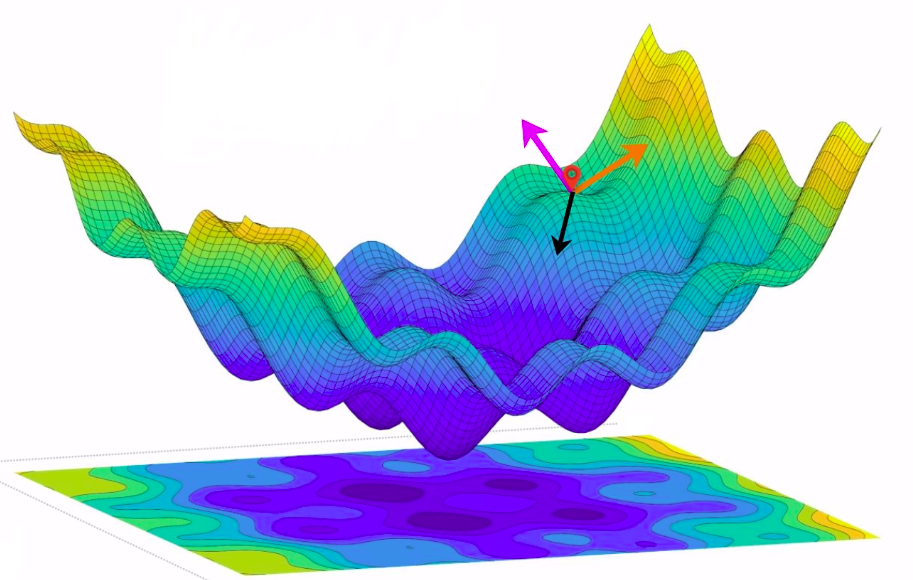
\includegraphics[width=0.8\linewidth]{3dg}};
	\end{tikzpicture}
\end{center}
%%%%%%%%%%%%%%%%%%%%%%%%%%%%%%%%%%%%%%%%%%%%%%%%%%%%%%%%%%%%%%%%%%%%%%%%%%%%%%%%%%%%%%%%%%%%%%%%%%%%%%%%%%%%%%%
%%%%%%%%%%%%%%%%%%%%%%%%%%%%%%%%%%%%%%%%%%%%%%%%%%%%%%%%%%%%%%%%%%%%%%%%%%%%%%%%%%%%%%%%%%%%%%%%%%%%%%%%%%%%%%%
\subsection{ La Función de Activación Sigmoide}	
%%%%%%%%%%%%%%%%%%%%%%%%%%%%%%%%%%%%%%%%%%%%%%%%%%%%%%%%%%%%%%%%%%%%%%%%%%%%%%%%%%%%%%%%%%%%%%%%%%%%%%%%%%%%%%%
%%%%%%%%%%%%%%%%%%%%%%%%%%%%%%%%%%%%%%%%%%%%%%%%%%%%%%%%%%%%%%%%%%%%%%%%%%%%%%%%%%%%%%%%%%%%%%%%%%%%%%%%%%%%%%%
Dicha función se define como
\begin{equation}
	\sigma(x)=\dfrac{1}{1+e^{-x}}.
\end{equation}
Cuya derivada es
\begin{eqnarray*}
	\sigma'(x)&=&\dfrac{d}{dx}(1+e^{-x})^{-1}\\
	&=&-(1+e^{-x})^{-2}(-e^{-x})\\
	&=&\dfrac{e^{-x}}{(1+e^{-x})^{2}}\\
	&=&\dfrac{1+e^{-x}-1}{(1+e^{-x})^{2}}\\
	&=&\dfrac{1}{1+e^{-x}}-\dfrac{1}{(1+e^{-x})^{2}}\\
	&=&\sigma(x)-\sigma^{2}(x)\\
	&=&\sigma(x)(1-\sigma(x)).
\end{eqnarray*}

La derivada de la función sigmoide queda en términos de ella misma, para la capa oculta el argumento de la función sigmoide es 
\[ h_{i_1} =\displaystyle\sum_{i_0} x_{i_0} w_{i_1}+\theta_{i_1}. \]
Entonces, para la derivada, se tiene 
%%%%%%%%%%%%%%%%%%%%%%%%%%%%%%%%%%%%%%%%%%%%%%%%%%%%%%%%%%%%%%%%%%%%%%%%%%%%%%%%%%%%%%%%%%%%%%%%%%%%%%%%%%%%%%%%%%%%%%%%%%%%%%%%%%%%%%%%%%%%%%
\begin{align}\label{dersig1}
	\sigma'(h_{i_1})=&\sigma(h_{i_1})(1-\sigma(h_{i_1}))\nonumber\\
	=&v_{i_1} (1-v_{i_1}).
\end{align}
%%%%%%%%%%%%%%%%%%%%%%%%%%%%%%%%%%%%%%%%%%%%%%%%%%%%%%%%%%%%%%%%%%%%%%%%%%%%%%%%%%%%%%%%%%%%%%%%%%%%%%%%%%%%%%%%%%%%%%%%%%%%%%%%%%%%%%%%%%%%%%

Por lo tanto, la derivada de la función sigmoide en $ h_{i_1} $ queda en términos de la salida de la neurona con etiqueta $ i_1 $. Análogamente para $ h_{i_2} $ se tiene
\begin{align}\label{dersig2}
	\sigma'(h_{i_2})&=\sigma(h_{i_2})(1-\sigma(h_{i_2}))\nonumber\\
	&=y_{i_2} (1-y_{i_2}).
\end{align}
%%%%%%%%%%%%%%%%%%%%%%%%%%%%%%%%%%%%%%%%%%%%%%%%%%%%%%%%%%%%%%%%%%%%%%%%%%%%%%%%%%%%%%%%%%%%%%%%%%%%%%%%%%%%%%%%%%%%%%%%%%%%%%%%%%%%%%%%%%%%%%%%%%%%%%%%%%%%%%%%%%%%%%%%%%%%%%%%%%%%%%%%%%%%%%%%%%%%%%%%%%%%%%%%%%%%%%%%%%%%%%%%%%%%%%%%%%%%%%%%%%%%%%%%%%%%%%%%%%%%%%%%%%%%%%%%%%%%%%%%%%%%

La funci\'on $ E(\hat{w})=\dfrac{1}{2}\displaystyle\sum_{i_2} (y_{i_2}-y_{i_2}^d)^2 $ depende de los pesos. El objetivo es encontrar el vector gradiente de la función de error cuadrático, por lo que se debe calcular la derivada parcial de $ E $ con respecto a cada peso.
%%%%%%%%%%%%%%%%%%%%%%%%%%%%%%%%%%%%%%%%%%%%%%%%%%%%%%%%%%%%%%%%%%%%%%%%%%%%%%%%%%%%%%%%%%%%%%%%%%%%%%%%%%%%%%%
%%%%%%%%%%%%%%%%%%%%%%%%%%%%%%%%%%%%%%%%%%%%%%%%%%%%%%%%%%%%%%%%%%%%%%%%%%%%%%%%%%%%%%%%%%%%%%%%%%%%%%%%%%%%%%%
\subsection{De la Capa de Salida a la Capa Oculta }
%%%%%%%%%%%%%%%%%%%%%%%%%%%%%%%%%%%%%%%%%%%%%%%%%%%%%%%%%%%%%%%%%%%%%%%%%%%%%%%%%%%%%%%%%%%%%%%%%%%%%%%%%%%%%%%
%%%%%%%%%%%%%%%%%%%%%%%%%%%%%%%%%%%%%%%%%%%%%%%%%%%%%%%%%%%%%%%%%%%%%%%%%%%%%%%%%%%%%%%%%%%%%%%%%%%%%%%%%%%%%%%
\noindent
Para calcular la derivada de $ E $ con respecto a un peso fijo que está entre la capa oculta y la capa de salida, se tiene
\begin{eqnarray}
	\dfrac{\partial E}{\partial w_{i_1 i_2}}&=&\dfrac{\partial E}{\partial y_{i_2}}\dfrac{\partial y_{i_2}}{\partial h_{i_2}} \dfrac{\partial h_{i_2}}{\partial w_{i_1 i_2}},
\end{eqnarray}
que representa retroceder de la última capa hacia la capa oculta. Se procede a realizar los cálculos.
\begin{center}
	\definecolor{ffqqqq}{rgb}{1,0,0}
	\definecolor{aqaqaq}{rgb}{0.6274509803921568,0.6274509803921568,0.6274509803921568}
	\definecolor{cqcqcq}{rgb}{0.7529411764705882,0.7529411764705882,0.7529411764705882}
	\begin{tikzpicture}[line cap=round,line join=round,>=triangle 45,x=1cm,y=1cm]
		\clip(2.8256391446426483,4) rectangle (12.158191550649723,7.974298823814763);
		\draw [line width=1pt] (4,6) circle (1cm);
		\draw [line width=1pt] (8,6) circle (1cm);
		\draw [->,line width=1pt] (5,6) -- (7,6);
		\draw [->,line width=1pt,color=aqaqaq] (5.393919298579168,-0.0808549699819415) -- (7.606080701420833,5.080854969981942);
		\draw [->,line width=1pt] (4.707106781186548,2.707106781186548) -- (7.292893218813452,5.292893218813452);
		\draw [->,line width=1pt] (11,6) -- (9,6);
		\draw [line width=1pt] (8,7)-- (8,5);
		\draw [shift={(8,6)},line width=1pt,fill=ffqqqq,fill opacity=0.35]  plot[domain=1.5707963267948965:4.71238898038469,variable=\t]({1*1*cos(\t r)+0*1*sin(\t r)},{0*1*cos(\t r)+1*1*sin(\t r)});
		\begin{scriptsize}
			\draw[color=black] (3.93,6.117589156108573) node {$v_{i_1}$};
			\draw[color=black] (8.4,6.117589156108573) node {$y_{i_2}$};
			\draw[color=black] (6.212364696880922,6.335385011557979) node {$w_{i_1 i_2}$};
			\draw[color=black] (10.002012581700597,6.226487083833276) node {$E$};
			\draw[color=black] (7.5,6.117589156108573) node {$h_{i_2}:\Sigma $};
		\end{scriptsize}
	\end{tikzpicture}
\end{center}

El error con respecto a la salida es
\begin{equation}\label{so1}
	\begin{array}{lll}
		\dfrac{\partial E}{\partial y_{i_2}}&=&\dfrac{\partial }{y_{i_2}}\left( \dfrac{1}{2}\displaystyle\sum_{i_2} (y_{i_2}-y_{i_2}^d)^2 \right)\\
		&=&\dfrac{1}{2} \dfrac{\partial}{\partial y_{i_2}}\left(\displaystyle\sum_{i_2} (y_{i_2}-y_{i_2}^d)^2 \right) \\
		&=&\dfrac{1}{2} 2 (y_{i_2}-y_{i_2}^d)\dfrac{\partial }{\partial y_{i_2}} (y_{i_2}-y_{i_2}^d)\\
		&=&\dfrac{1}{2} 2 (y_{i_2}-y_{i_2}^d)\left( \dfrac{\partial y_{i_2}}{\partial y_{i_2}} - \dfrac{\partial y_{i_2}^d}{\partial y_{i_2}} \right)\\
		&=&\dfrac{1}{2} 2 (y_{i_2}-y_{i_2}^d)\left( 1-0 \right)\\
		&=&y_{i_2}-y_{i_2}^d.\\
	\end{array}
\end{equation}

La salida con respecto a la suma es
\begin{equation}\label{so2}
	\begin{array}{lll}
		\dfrac{\partial y_{i_2}}{\partial h_{i_2}}&=&\dfrac{\partial} {\partial h_{i_2}} \sigma(h_{i_2})\\
		&=&\underbrace{\sigma(h_{i_2})(1-\sigma(h_{i_2}))}_{\ref{dersig2}} \\
		&=&y_{i_2}(1-y_{i_2}).\\
	\end{array}
\end{equation}

La suma con respecto al peso es
\begin{equation}\label{so3}
	\begin{array}{lll}
		\dfrac{\partial h_{i_2}}{\partial w_{i_1 i_2}}&=&\dfrac{\partial}{\partial w_{i_1 i_2}} \left(  \displaystyle\sum_{i_1} w_{i_1 i_2} v_{i_1} + \theta_{i_1} \right)\\
		&=&v_{i_1}.\\
	\end{array}
\end{equation}

De lo anterior se tiene que
\begin{eqnarray*}
	\dfrac{\partial E}{\partial w_{i_1 i_2}}&=&\dfrac{\partial E}{\partial y_{i_2}}\dfrac{\partial y_{i_2}}{\partial h_{k}}\dfrac{\partial h_{i_2}}{\partial w_{i_1 i_2}}\\
	&=&\underbrace{(y_{i_2}-y_{i_2}^d)}_{(\ref{so1})}\underbrace{y_{i_2}(1-y_{i_2})}_{(\ref{so2})}v_{i_1}.
\end{eqnarray*}

Las primeras dos componentes de la última expresión dependen de la neurona con etiqueta $ i_2 $, por motivos de notación se nombrará como
\begin{equation}\label{deltao}
	\delta_{i_2}= y_{i_2}(1-y_{i_2})(y_{i_2}-y_{i_2}^d).
\end{equation}

Por lo que
\[ \dfrac{\partial E}{\partial y_{i_2}}= v_{i_1}\delta_{i_2}. \]

%%%%%%%%%%%%%%%%%%%%%%%%%%%%%%%%%%%%%%%%%%%%%%%%%%%%%%%%%%%%%%%%%%%%%%%%%%%%%%%%%%%%%%%%%%%%%%%%%%%%%%%%%%%%%%%
%%%%%%%%%%%%%%%%%%%%%%%%%%%%%%%%%%%%%%%%%%%%%%%%%%%%%%%%%%%%%%%%%%%%%%%%%%%%%%%%%%%%%%%%%%%%%%%%%%%%%%%%%%%%%%%
\subsection{De la Capa Oculta a la Capa de Entrada}
%%%%%%%%%%%%%%%%%%%%%%%%%%%%%%%%%%%%%%%%%%%%%%%%%%%%%%%%%%%%%%%%%%%%%%%%%%%%%%%%%%%%%%%%%%%%%%%%%%%%%%%%%%%%%%%
%%%%%%%%%%%%%%%%%%%%%%%%%%%%%%%%%%%%%%%%%%%%%%%%%%%%%%%%%%%%%%%%%%%%%%%%%%%%%%%%%%%%%%%%%%%%%%%%%%%%%%%%%%%%%%%
\begin{center}
	\definecolor{ffqqqq}{rgb}{1,0,0}
	\definecolor{cqcqcq}{rgb}{0.7529411764705882,0.7529411764705882,0.7529411764705882}
	\definecolor{ududff}{rgb}{0.30196078431372547,0.30196078431372547,1}
	\begin{tikzpicture}[line cap=round,line join=round,>=triangle 45,x=0.7cm,y=0.7cm]
		\clip(-1.7738885880748125,0.4884263451511421) rectangle (9.612366755477316,7.599174511172158);
		\draw [line width=1pt] (0,6) circle (0.7cm);
		\draw [line width=1pt] (4,6) circle (0.7cm);
		\draw [line width=1pt] (8,6) circle (0.7cm);
		\draw [line width=1pt] (8,2) circle (0.7cm);
		\draw [->,line width=1pt] (1,6) -- (3,6);
		\draw [->,line width=1pt] (5,6) -- (7,6);
		\draw [->,line width=1pt] (4.707106781186548,5.292893218813452) -- (7.292893218813452,2.707106781186548);
		\draw [shift={(4,6)},line width=1pt,color=ffqqqq,fill=ffqqqq,fill opacity=0.5]  plot[domain=1.5707963267948965:4.71238898038469,variable=\t]({1*1*cos(\t r)+0*1*sin(\t r)},{0*1*cos(\t r)+1*1*sin(\t r)});
		\draw [line width=1pt] (4,7)-- (4,5);
		\draw [shift={(4,6)},line width=1pt]  plot[domain=1.5707963267948965:4.71238898038469,variable=\t]({1*1*cos(\t r)+0*1*sin(\t r)},{0*1*cos(\t r)+1*1*sin(\t r)});
		\draw [shift={(4,6)},line width=1pt]  plot[domain=1.5707963267948965:4.71238898038469,variable=\t]({1*1*cos(\t r)+0*1*sin(\t r)},{0*1*cos(\t r)+1*1*sin(\t r)});
		\draw [shift={(8,6)},line width=1pt,color=ffqqqq,fill=ffqqqq,fill opacity=0.5]  plot[domain=1.5707963267948965:4.71238898038469,variable=\t]({1*1*cos(\t r)+0*1*sin(\t r)},{0*1*cos(\t r)+1*1*sin(\t r)});
		\draw [line width=1pt] (8,7)-- (8,5);
		\draw [shift={(8,6)},line width=1pt]  plot[domain=1.5707963267948965:4.71238898038469,variable=\t]({1*1*cos(\t r)+0*1*sin(\t r)},{0*1*cos(\t r)+1*1*sin(\t r)});
		\draw [shift={(8,6)},line width=1pt]  plot[domain=1.5707963267948965:4.71238898038469,variable=\t]({1*1*cos(\t r)+0*1*sin(\t r)},{0*1*cos(\t r)+1*1*sin(\t r)});
		\draw [shift={(8,2)},line width=1pt,color=ffqqqq,fill=ffqqqq,fill opacity=0.5]  plot[domain=1.5707963267948965:4.71238898038469,variable=\t]({1*1*cos(\t r)+0*1*sin(\t r)},{0*1*cos(\t r)+1*1*sin(\t r)});
		\draw [line width=1pt] (8,3)-- (8,1);
		\draw [shift={(8,2)},line width=1pt]  plot[domain=1.5707963267948965:4.71238898038469,variable=\t]({1*1*cos(\t r)+0*1*sin(\t r)},{0*1*cos(\t r)+1*1*sin(\t r)});
		\draw [shift={(8,2)},line width=1pt]  plot[domain=1.5707963267948965:4.71238898038469,variable=\t]({1*1*cos(\t r)+0*1*sin(\t r)},{0*1*cos(\t r)+1*1*sin(\t r)});
		\begin{scriptsize}
			\draw[color=black] (-0.04375750564167273,6.1996705727642) node {$x_{i_0}$};
			\draw[color=black] (1.8,6.272136796112185) node {$w_{i_0 i_1}$};
			\draw[color=black] (3.6252039942465845,6.190612294845701) node {$h_{i_1}$};
			\draw[color=black] (4.6,6.190612294845701) node {$v_{i_1} $};
			\draw[color=black] (7.6,6.190612294845701) node {$h_{1_2}$};
			\draw[color=black] (8.5,6.1906) node {$y_{1_2}$};
			\draw[color=black] (7.6,2) node {$h_{2_2}$};
			\draw[color=black] (8.5,2) node {$y_{2_2}$};
			\draw[color=black] (5.7,6.281195074030682) node {$w_{i_1 1_2}$};
			\draw[color=black] (6.8,4.125324929428133) node {$w_{i_1 2_2}$};
		\end{scriptsize}
	\end{tikzpicture}
\end{center}

El error para $w_{i_0 i_1} $ depende del error de las conexiones de la capa anterior.
\begin{eqnarray*}
	\dfrac{\partial E}{\partial w_{i_0 i_1}}&=&\dfrac{\partial}{\partial w_{i_0 i_1}}\dfrac{1}{2}\displaystyle\sum_{i_2} (y_{i_2}-y_{i_2}^d)^2\\
	&=&\dfrac{1}{2}\cdot 2 \displaystyle\sum_{i_2}(y_{i_2}-y_{i_2}^d) \dfrac{\partial }{\partial w_{i_0 i_1}}(y_{i_2}-y_{i_2}^d)\\
	&=&\displaystyle\sum_{i_2} (y_{i_2}-y_{i_2}^d) \left(\dfrac{\partial y_{i_2}}{\partial w_{i_0 i_1}}-\dfrac{\partial y_{i_2}^d}{\partial w_{i_0 i_1}}\right)\\
	&=&\displaystyle\sum_{i_2} (y_{i_2}-y_{i_2}^d) \left(\dfrac{\partial y_{i_2}}{\partial w_{i_0 i_1}}-0\right)\\
	&=&\displaystyle\sum_{i_2} (y_{i_2}-y_{i_2}^d) \dfrac{\partial y_{i_2}}{\partial w_{i_0 i_1}}\\
	&=&\displaystyle\sum_{i_2}(y_{i_2}-y_{i_2}^d) \dfrac{\partial y_{i_2}}{\partial h_{i_2}}\dfrac{\partial h_{i_2}}{\partial v_{i_1}}\dfrac{\partial v_{i_1}}{\partial w_{i_0 i_1}}\\
	&=&\underbrace{\dfrac{\partial v_{i_1}}{\partial w_{i_0 i_1}}}_{\ref{hi1}}\displaystyle\sum_{i_2} (y_{i_2}-y_{i_2}^d) \underbrace{\dfrac{\partial y_{i_2}}{\partial h_{i_2}}}_{\ref{dersig2}}\dfrac{\partial h_{i_2}}{\partial v_{i_1}}. 
\end{eqnarray*} 

Calculando las derivadas
\begin{equation}\label{hi1}
	\begin{array}{lll}
		\dfrac{\partial v_{i_1}}{\partial w_{i_0 i_1}} &=& \dfrac{\partial v_{i_1}}{\partial  h_{i_1}}\dfrac{\partial h_{i_1}}{\partial  \partial w_{i_0 i_1}}  \\
		&=& \underbrace{\dfrac{\partial }{\partial  h_{i_1}} \sigma (h_{i_1})}_{\ref{dersig1}} \dfrac{\partial }{\partial  w_{i_0 i_1}}  \displaystyle\sum_{i_1} \left( w_{i_0 i_1} x_{i_0} + \theta_{i_1}\right)\\
		&=& v_{i_1} (1-v_{i_1}) x_{i_0}.
	\end{array}
\end{equation}	

\begin{equation}
	\begin{array}{lll}
		\dfrac{\partial h_{i_2}}{\partial v_{i_1}} &=&  \dfrac{\partial }{\partial v_{i_1}} \displaystyle\sum_{i_2} \left(w_{i_0 i_1} v_{i_1} + \theta_{i_2}\right)\\
		&=& w_{i_0 i_1}.
	\end{array}
\end{equation}
Así que para la capa oculta se obtiene
\begin{eqnarray*}
	\dfrac{\partial E}{\partial w_{i_0 i_1}}&=&\dfrac{\partial v_{i_1}}{\partial w_{i_0 i_1}}\displaystyle\sum_{i_2} (y_{i_2}-y_{i_2}^d) \dfrac{\partial y_{i_2}}{\partial h_{i_2}}\dfrac{\partial h_{i_2}}{\partial v_{i_1}}\\
	&=&\underbrace{v_{i_1} (1-v_{i_1}) x_{i_0}}_{(\ref{hi1})} \displaystyle\sum_{i_2} \underbrace{(y_{i_2}-y_{i_2}^d) \overbrace{y_{i_2} (1-y_{i_2})}^{(\ref{so2})}}_{(\ref{deltao})} w_{i_1 i_2}\\
	&=&v_{i_1}(1-v_{i_1}) x_{i_0} \displaystyle\sum_{i_2} \delta_{i_2} w_{i_1 i_2}\\
	&=&x_{i_0} v_{i_1} (1-v_{i_1})\displaystyle\sum_{i_2} \delta_{i_2}w_{i_1 i_2}.
\end{eqnarray*}

Si se define 
\[ \delta_{i_1} = v_{i_1} (1-v_{i_1})  \displaystyle\sum_{i_2} \delta_{i_2} w_{i_1 i_2}, \]
entonces 
\[ \dfrac{\partial E}{\partial w_{i_0 i_1}} = x_{i_0} \delta_{i_1}. \]
\textbf{Incorporando el Bias}

Para las neuronas de la última capa con sesgo $ (\theta_{i_2}) $, se tiene que 
\begin{eqnarray*}
	\dfrac{\partial E}{\partial \theta_{i_2}}&=&\dfrac{\partial E}{\partial y_{i_2}}\dfrac{\partial y_{i_2}}{\partial h_{i_2}}\dfrac{\partial h_{i_2}}{\partial \theta_{i_2}}\\
	&=& \delta_{i_2} \dfrac{\partial h_{i_2}}{\partial \theta_{i_2}}\\
	&=& \delta_{i_2}\dfrac{\partial}{\partial \theta_{i_2}}\sum_{i_2}\left( w_{i_1 i_2} v_{i_1} + \theta_{i_2}\right)\\
	&=& \delta_{i_2}.
\end{eqnarray*}
%%%%%%%%%%%%%%%%%%%%%%%%%%%%%%%%%%%%%%%%%%%%%%%%%%%%%%%%%%%%%%%%%%%%%%%%%%%%%%%%%%%%%%%%%%%%%%%%%%%%%%%%%%%%%%%
%%%%%%%%%%%%%%%%%%%%%%%%%%%%%%%%%%%%%%%%%%%%%%%%%%%%%%%%%%%%%%%%%%%%%%%%%%%%%%%%%%%%%%%%%%%%%%%%%%%%%%%%%%%%%%%
\subsection{El Algoritmo}
%%%%%%%%%%%%%%%%%%%%%%%%%%%%%%%%%%%%%%%%%%%%%%%%%%%%%%%%%%%%%%%%%%%%%%%%%%%%%%%%%%%%%%%%%%%%%%%%%%%%%%%%%%%%%%%
%%%%%%%%%%%%%%%%%%%%%%%%%%%%%%%%%%%%%%%%%%%%%%%%%%%%%%%%%%%%%%%%%%%%%%%%%%%%%%%%%%%%%%%%%%%%%%%%%%%%%%%%%%%%%%%
\begin{enumerate}
	\item Crear una red neuronal y cargar los datos de entrenamiento. 
	
	\textbf{Nota. }La red neuronal que se crea tiene un número fijo de neuronas para la capa de entrada y la capa de salida (dependen del conjunto de aprendizaje). Sin embargo, el número de neuronas en la capa oculta queda libre.
	\item Generar pesos aleatorios tanto para las conexiones entre neuronas como para los bias.
	\item Para cada nodo en la capa de salida, calcular
	\[ \delta_{i_2}= y_{i_2}(1-y_{i_2})(y_{i_2}-y_{i_2}^d). \]
	\item Para cada nodo en la capa oculta, calcular
	\[ \delta_{i_1} = v_{i_1} (1-v_{i_1})  \displaystyle\sum_{i_2} \delta_{i_2} w_{i_1 i_2}. \]
	\item Actualizar los pesos como sigue
	\begin{eqnarray*}
		\Delta w_{i_1 i_2}     &=&-\eta \delta_{i_2} v_{i_1},\\
		\Delta w_{i_0 i_1}     &=&-\eta \delta_{i_1} x_{i_0},\\
		\Delta \theta_{i_2}    &=&-\eta \delta_{i_2},\\
		\Delta \theta_{i_1}    &=&-\eta \delta_{i_1},\\
	\end{eqnarray*}
	para un $ 0<\eta\leq 1 $ (este número también se desconoce y debe ajustarse según la experimentación). Luego aplicar
	\begin{eqnarray*}
		w+\Delta w    	    &\to&w \\
		\theta+\Delta \theta&\to&\theta.
	\end{eqnarray*}
\end{enumerate}

Aunque este algoritmo ha mostrado eficiencia, los recursos computacionales son limitados y para grandes conjuntos de datos, requiere un tiempo computacional exhaustivo. Por otro lado, como los pesos se dan de manera aleatoria se podría comenzar en un mínimo local del espacio pesos-función de error que nunca cumpla con los parámetros elegidos.

De aquí la importancia de buscar nuevos algoritmos para entrenar a redes neuronales. En la siguiente  sección se muestra un algoritmo que translada el problema de encontrar los pesos de una red neuronal a un problema de control cuya solución corresponde a la solución de una ecuación diferencial parcial conocida.



%%%%%%%%%%%%%%%%%%%%%%%%%%%%%%%%%%%%%%%%%%%%%%%%%%%%%%%%%%%%%%%%%%%%%%%%%%%%%%%%%%
\selectlanguage{spanish}
\bibliographystyle{acm}
\bibliography{ref}

\end{document}